% !TeX program = xelatex

\documentclass[type = bachelor]{whu-thesis}

\whusetup{
	info = {
		title      = {小型化冷原子真空计量系统\\磁光阱装载实验},
		title*     = {A prototype of a portable cold-atom vacuum gauge},
		department = {物理学院},
		department* = {Department of Physics},
		author     = {陈瑞西},
		author*    = {Chen Ruixi},
		student-id = {2022302191455},
		supervisor = {江开军研究员},
		supervisor* = {Jiang Kaijun},
		supervisor-outer = {张立},
		academic-title = {研究员},
		academic-title* = {},
		academic-title-outer = {},
		subject = {},
		major   = {物理学},
		major* = {Physics},
		research-area = {原子分子光物理},
		research-area* = {},
		year = 2026,
		keywords = {冷原子真空计量；磁光阱；激光冷却},
		keywords* = {Cold atom vacuum metrology;Magneto-optical trap;Laser cooling},
		month = 5,
		clc = O175.29,
		udc = 517.9,
	},
	style = {
		% footnote-style = libertinus-sans,
		font = times,
		math-font = default,
		cjk-font = windows,
		% library,
		% cjk-fakefont = true,
		bib-backend = bibtex,
		% bib-style = numerical,
		bib-resource = {ref/CAVS},
		bachelor-encover = false, % 显示英文封面
		license = false
	}
}

% 宏包引入
\usepackage{physics}
\usepackage{amsmath}
%% 允许公式换页
\allowdisplaybreaks[4]
\usepackage{extarrows}
\usepackage{annotate-equations}
\usepackage{cancel}
\usepackage{slashed}
\usepackage{tcolorbox}
\usepackage{shuffle}
\usepackage{simpler-wick}
\usepackage{mathtools}
\usepackage{braket}
\usepackage{siunitx}   % 标准单位排版包
\usepackage[version=4]{mhchem}    % 规范化学分子式排版
%自定义命令
%% 实现双重尖括号
\makeatletter
\newsavebox{\@brx}
\newcommand{\llangle}[1][]{\savebox{\@brx}{\(\m@th{#1\langle}\)}%
	\mathopen{\copy\@brx\kern-0.5\wd\@brx\usebox{\@brx}}}
\newcommand{\rrangle}[1][]{\savebox{\@brx}{\(\m@th{#1\rangle}\)}%
	\mathclose{\copy\@brx\kern-0.5\wd\@brx\usebox{\@brx}}}
\makeatother
%% 重要定理框注
\newenvironment{boxedtext}[1][定理] % 定义带参数的环境，参数数量为1（定理名称）
{
	\begin{tcolorbox}[
		colback=gray!10,                % 灰色背景
		colframe=black,                 % 黑色边框
		arc=1mm,                        % 圆角弧度
		auto outer arc,                 % 自动外弧
		boxrule=0.5pt,                  % 边框线宽
		title={\bfseries #1},           % 定理名称参数（加粗显示）
		coltitle=white,                 % 标题文字白色
		colbacktitle=black!70,          % 标题背景深灰色（非纯黑）
		]
	}
	{
	\end{tcolorbox}
}

\begin{document}
	%生成目录
	\tableofcontents
	% \listoffigures
	% \listoftables
	% 正文
	\mainmatter
	%\chapter{绪论}
\label{chap:1}
\section{研究背景与研究意义}

超高真空（Ultra-High Vacuum, UHV，通常指压力低于 $10^{-6}\,\mathrm{Pa}$ 的真空环境）是现代高端科学实验与先进制造技术的重要基础条件\cite{arpornthipVacuumpressureMeasurementUsing2012,成永军基于7Li冷原子操控的超高真空测量2024,贾文杰基于冷原子的量子真空计量技术研究进展2021,张苏钊基于磁光阱中6Li冷原子的真空度测量2022}。在基础科学领域，例如冷原子物理、量子信息技术、精密光谱测量以及基本常数测定等实验中，超高真空环境是获得长相干时间和高信噪比测量结果的前提条件\cite{barkerAccurateMeasurementLoss2023}。在粒子物理与加速器工程中，束流管道必须维持极低的气体密度，以减少粒子与残余气体分子的碰撞，从而避免能量损失及束流不稳定现象\cite{barkerPreciseQuantumMeasurement2022}。在航天推进系统、精密仪器制造以及表面科学分析（如扫描隧道显微镜、电子束曝光）等领域，稳定、可靠的超高真空测量同样发挥着关键作用\cite{barkerPreciseQuantumMeasurement2022}。因此，研发高精度、可溯源且对被测系统扰动较小的超高真空测量技术具有重要的现实意义和工程价值。

目前，超高真空测量领域广泛采用真空电离规作为主要测量手段，典型代表包括热阴极电离规和冷阴极电离规。然而，传统电离规在高精度测量与长期稳定运行方面仍存在若干固有局限，例如气体解吸效应、软 X 射线效应以及高温灯丝热辐射等问题\cite{bayardExtensionLowPressure1950}。这些因素会引入附加误差或背景信号，进而影响测量结果的准确性与系统运行的稳定性。

近年来发展起来的基于冷原子碰撞损失机制的真空测量技术，其核心思想在于利用冷原子与背景气体分子之间的弹性或非弹性碰撞这一内禀微观过程，实现对环境压强的量子化测量。在超高真空条件下，被俘获冷原子因与背景气体分子发生碰撞而逃逸出势阱，从而表现为原子数的指数衰减，其衰减速率 $\Gamma$ 与背景气体数密度 $n$ 之间满足线性关系
\[
n = \frac{\Gamma}{L},
\]
其中 $L$ 为损失率系数（loss-rate coefficient）。
结合理想气体状态方程
\[
P = nkT,
\]
可得到压强与原子损失率之间的直接关系\cite{barkerPreciseQuantumMeasurement2022}
\[
P = \frac{\Gamma}{L} k T.
\]

其中，损失率系数 $L$ 由原子—分子散射截面及相对速度分布决定，本质上仅依赖于微观相互作用势等基本物理参数，可通过第一性原理计算获得；玻尔兹曼常数 $k$ 为已知物理常数。因此，通过精确测量原子数衰减速率 $\Gamma$ 及环境温度 $T$，即可实现对环境压强 $P$ 的反演求解。

原子数衰减率的测量目前主要包含两种方法，其基本测量流程如下。首先，经过预冷却的原子蒸汽被囚禁于三维磁光阱中，衰减率测量过程可在磁光阱或磁阱内分别实施。第一种方法是在三维磁光阱中直接监测原子数的衰减过程，利用原子荧光强度表征原子数密度，通过获取荧光强度随时间的演化曲线，拟合得到原子数衰减速率$\Gamma$，如图\ref{fig:ch1-5}。该方法测量效率较高，能够快速获得衰减曲线，但原子与背景气体的碰撞截面计算较为复杂，现阶段仍缺乏精确的理论计算方法。

\begin{figure}[htbp] \centering 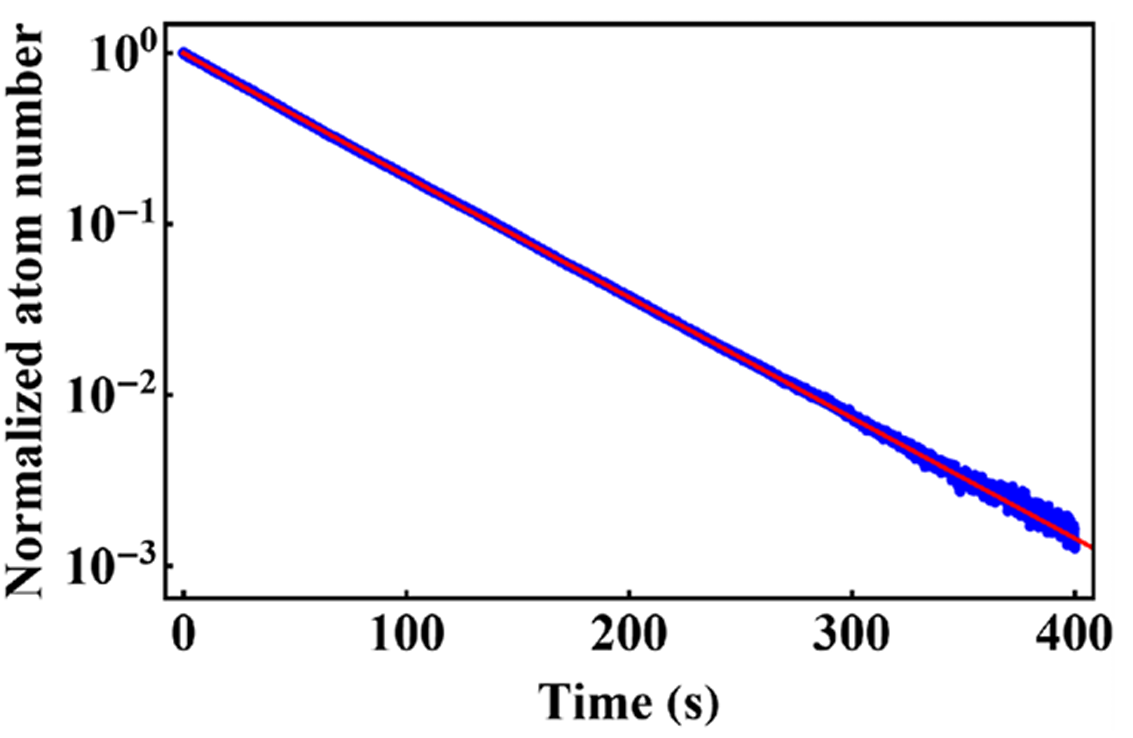
\includegraphics[width=0.5\linewidth]{figs/ch1-5.png} \caption{磁光阱中原子数衰减曲线\cite{zhangVacuumPressureMeasurement2023}} 
	\label{fig:ch1-5} 
\end{figure}

第二种方法则是将冷却后的原子从三维磁光阱装载至磁阱中，由于磁阱内不存在照射光束，原子无法产生荧光信号；待原子在磁阱中经历指定时间的数目衰减后，再将其重新装载回三维磁光阱进行荧光检测，通过对比不同时刻的荧光强度变化拟合出衰减速率$\Gamma$，如图\ref{fig:ch1-6}。此种方法的优势在于磁阱中原子与背景气体的碰撞截面物理图像明确、计算精度更高，不足之处是测量周期较长，需要对多个时间节点的原子数进行重复测量。

\begin{figure}[htbp] \centering 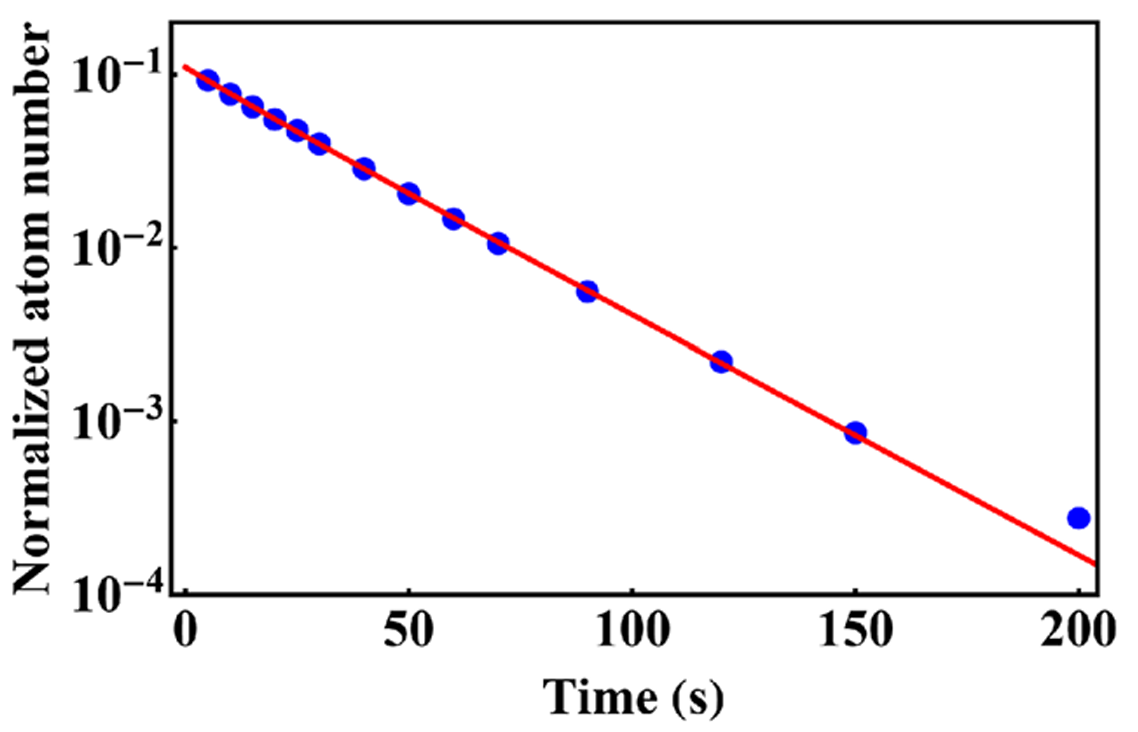
\includegraphics[width=0.5\linewidth]{figs/ch1-6.png} \caption{磁阱中原子数衰减曲线\cite{zhangVacuumPressureMeasurement2023}} 
	\label{fig:ch1-6} 
\end{figure}

由于该方法直接建立在微观散射动力学之上，避免了传统电离规中与电子发射、气体种类依赖等相关的系统误差来源，在原理上具有更高的准确度与长期稳定性。同时，其测量结果可溯源至基本物理常数与第一性原理计算，因而具备发展为新一代初级真空计量标准的潜力。


冷原子真空测量技术的发展可追溯至20世纪80年代激光冷却与俘获技术的突破。1987年磁光阱（Magneto-Optical Trap, MOT）的发明首次实现了对中性原子的稳定空间俘获，使原子样品能够在超高真空环境中长时间存留。随后研究逐步表明，原子俘获寿命与背景气体压强之间存在直接关联关系\cite{bjorkholmCollisionlimitedLifetimesAtom1988}，这一认识为基于碰撞损失机制的真空测量方法奠定了关键实验基础。

进入2010年代，随着激光系统稳定性的提升以及原子-分子碰撞截面计算精度的显著提高，相关研究由早期的定性关联分析逐步发展为定量模型构建，开始系统探索利用冷原子俘获寿命实现真空计量的可行性\cite{arpornthipVacuumpressureMeasurementUsing2012}。这一阶段标志着该技术从基础原子物理研究向计量应用方向的初步过渡。

美国国家标准与技术研究院（National Institute of Standards and Technology, NIST）在该领域开展了系统性研究，提出并实现了基于冷原子碰撞动力学的超高及极高真空量子标准体系。其核心思想是通过测量俘获原子的损失速率，并结合第一性原理计算得到的碰撞损失率系数，实现压力对基本物理常数的可溯源测量\cite{scherschligtDevelopmentNewUHV2017,barkerAccurateMeasurementLoss2023,barkerPreciseQuantumMeasurement2022,eckelEffectGlancingCollisions2025}。基于该原理，NIST构建了以铷原子为传感介质的实验室级量子真空计量装置，如图\ref{fig:ch1-1}所示。相关研究围绕碰撞截面的精确计算、原子损失模型修正、系统误差来源分析以及测量不确定度评定等关键问题展开，逐步建立了完整的量子真空计量框架。

\begin{figure}[htbp] \centering 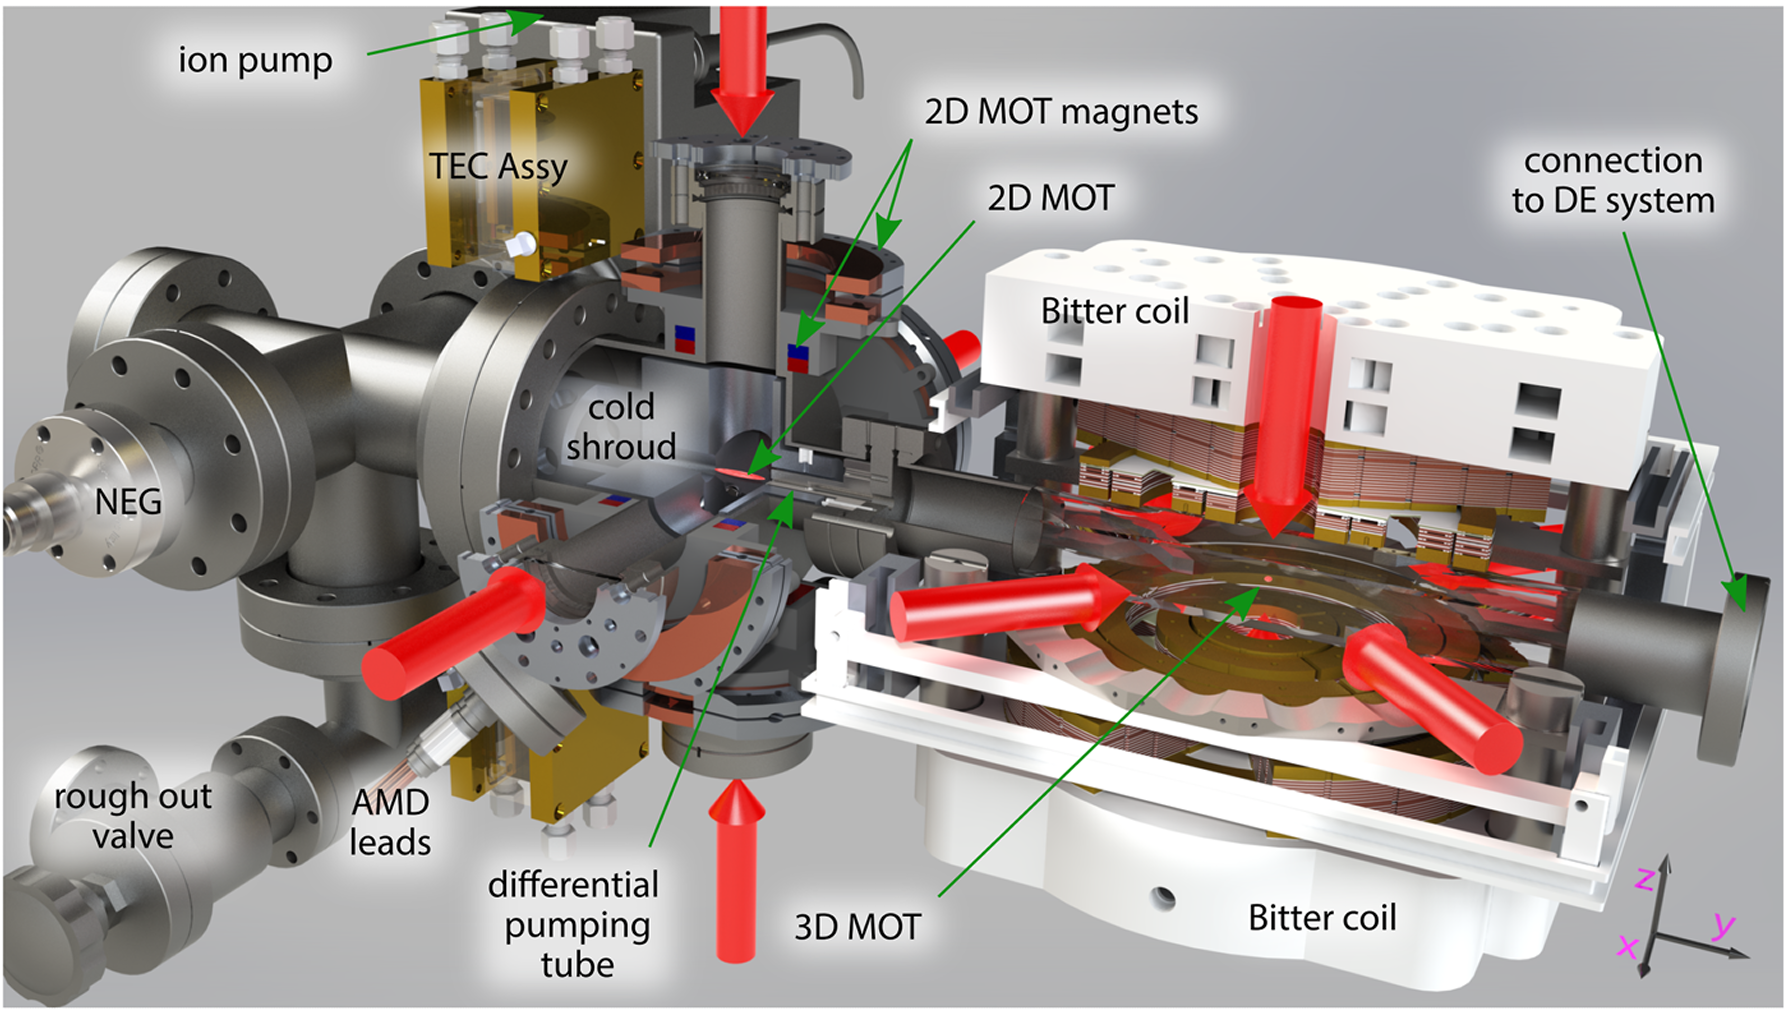
\includegraphics[width=0.5\linewidth]{figs/ch1-1.png} \caption{NIST实验室级量子真空计量装置\cite{barkerPreciseQuantumMeasurement2022}} 
\label{fig:ch1-1} 
\end{figure}

在工程实现方面，NIST进一步发展了基于锂原子的便携式冷原子真空标准装置\cite{barkerPreciseQuantumMeasurement2022,ehingerComparisonTwoMultiplexed2022}，如图\ref{fig:ch1-2}所示。通过引入紧凑型激光系统、永磁体磁场结构以及集成化光学模块设计，显著降低了系统体积与功耗，为现场应用与工程化部署提供了重要技术验证。

\begin{figure}[htbp] \centering 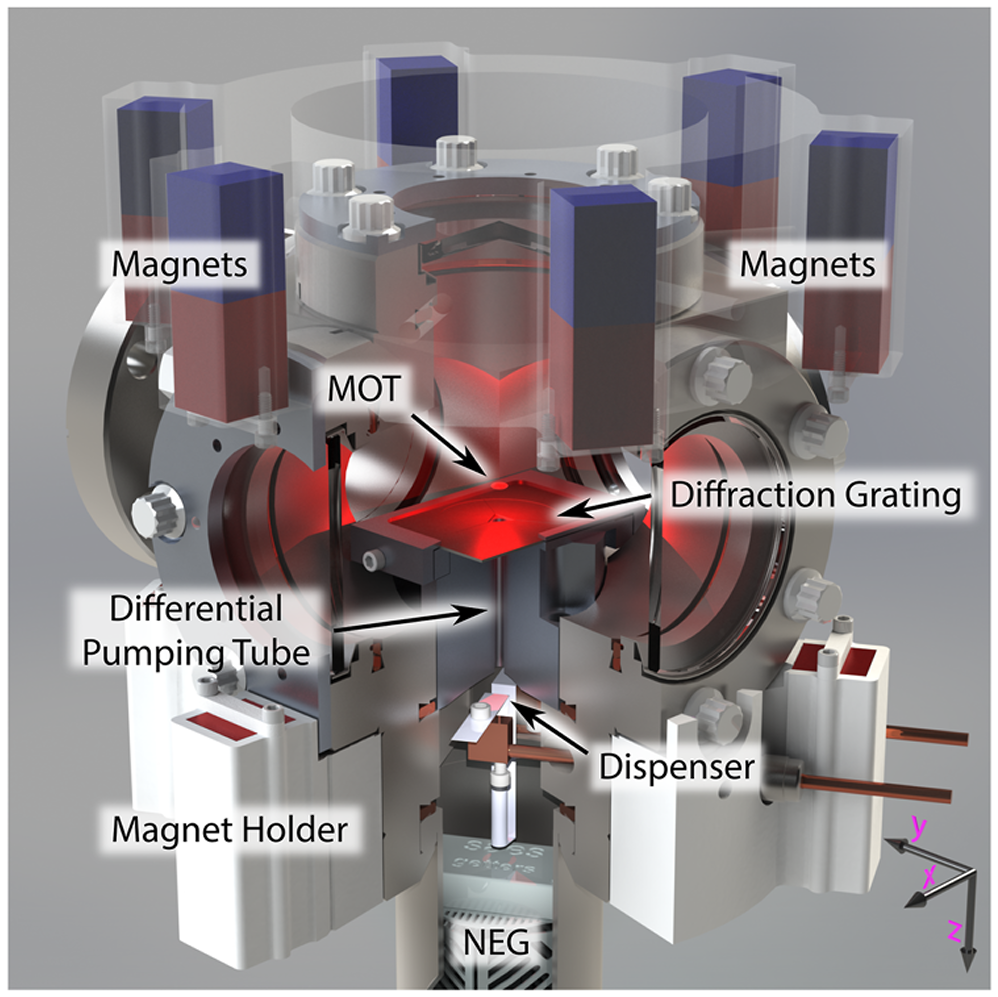
\includegraphics[width=0.5\linewidth]{figs/ch1-2.png} \caption{NIST基于锂原子的便携式冷原子真空标准装置\cite{barkerPreciseQuantumMeasurement2022}} \label{fig:ch1-2} \end{figure}

除NIST外，加拿大英属哥伦比亚大学（University of British Columbia, UBC）亦开展了系统研究，构建了基于铷原子的量子真空计量实验平台，如图\ref{fig:ch1-3}所示。其研究重点在于冷原子损失机制的精确建模以及多组分气体环境下的响应特性分析，同时对小型化冷原子真空计量装置进行了探索\cite{boothUniversalityQuantumDiffractive2019,shenDevelopmentColdAtom2022,shenRealizationUniversalQuantum2020,waldockProgressPortableColdatom2022}。此外，欧洲部分计量机构和研究团队亦对基于冷原子的量子真空计量方法开展了相关研究\cite{makhalovVacuumGaugeBased2017,halbeyDesignAdvancesDual2025}，为该技术纳入国际计量标准体系提供了重要的理论与实验支撑。

\begin{figure}[htbp] \centering 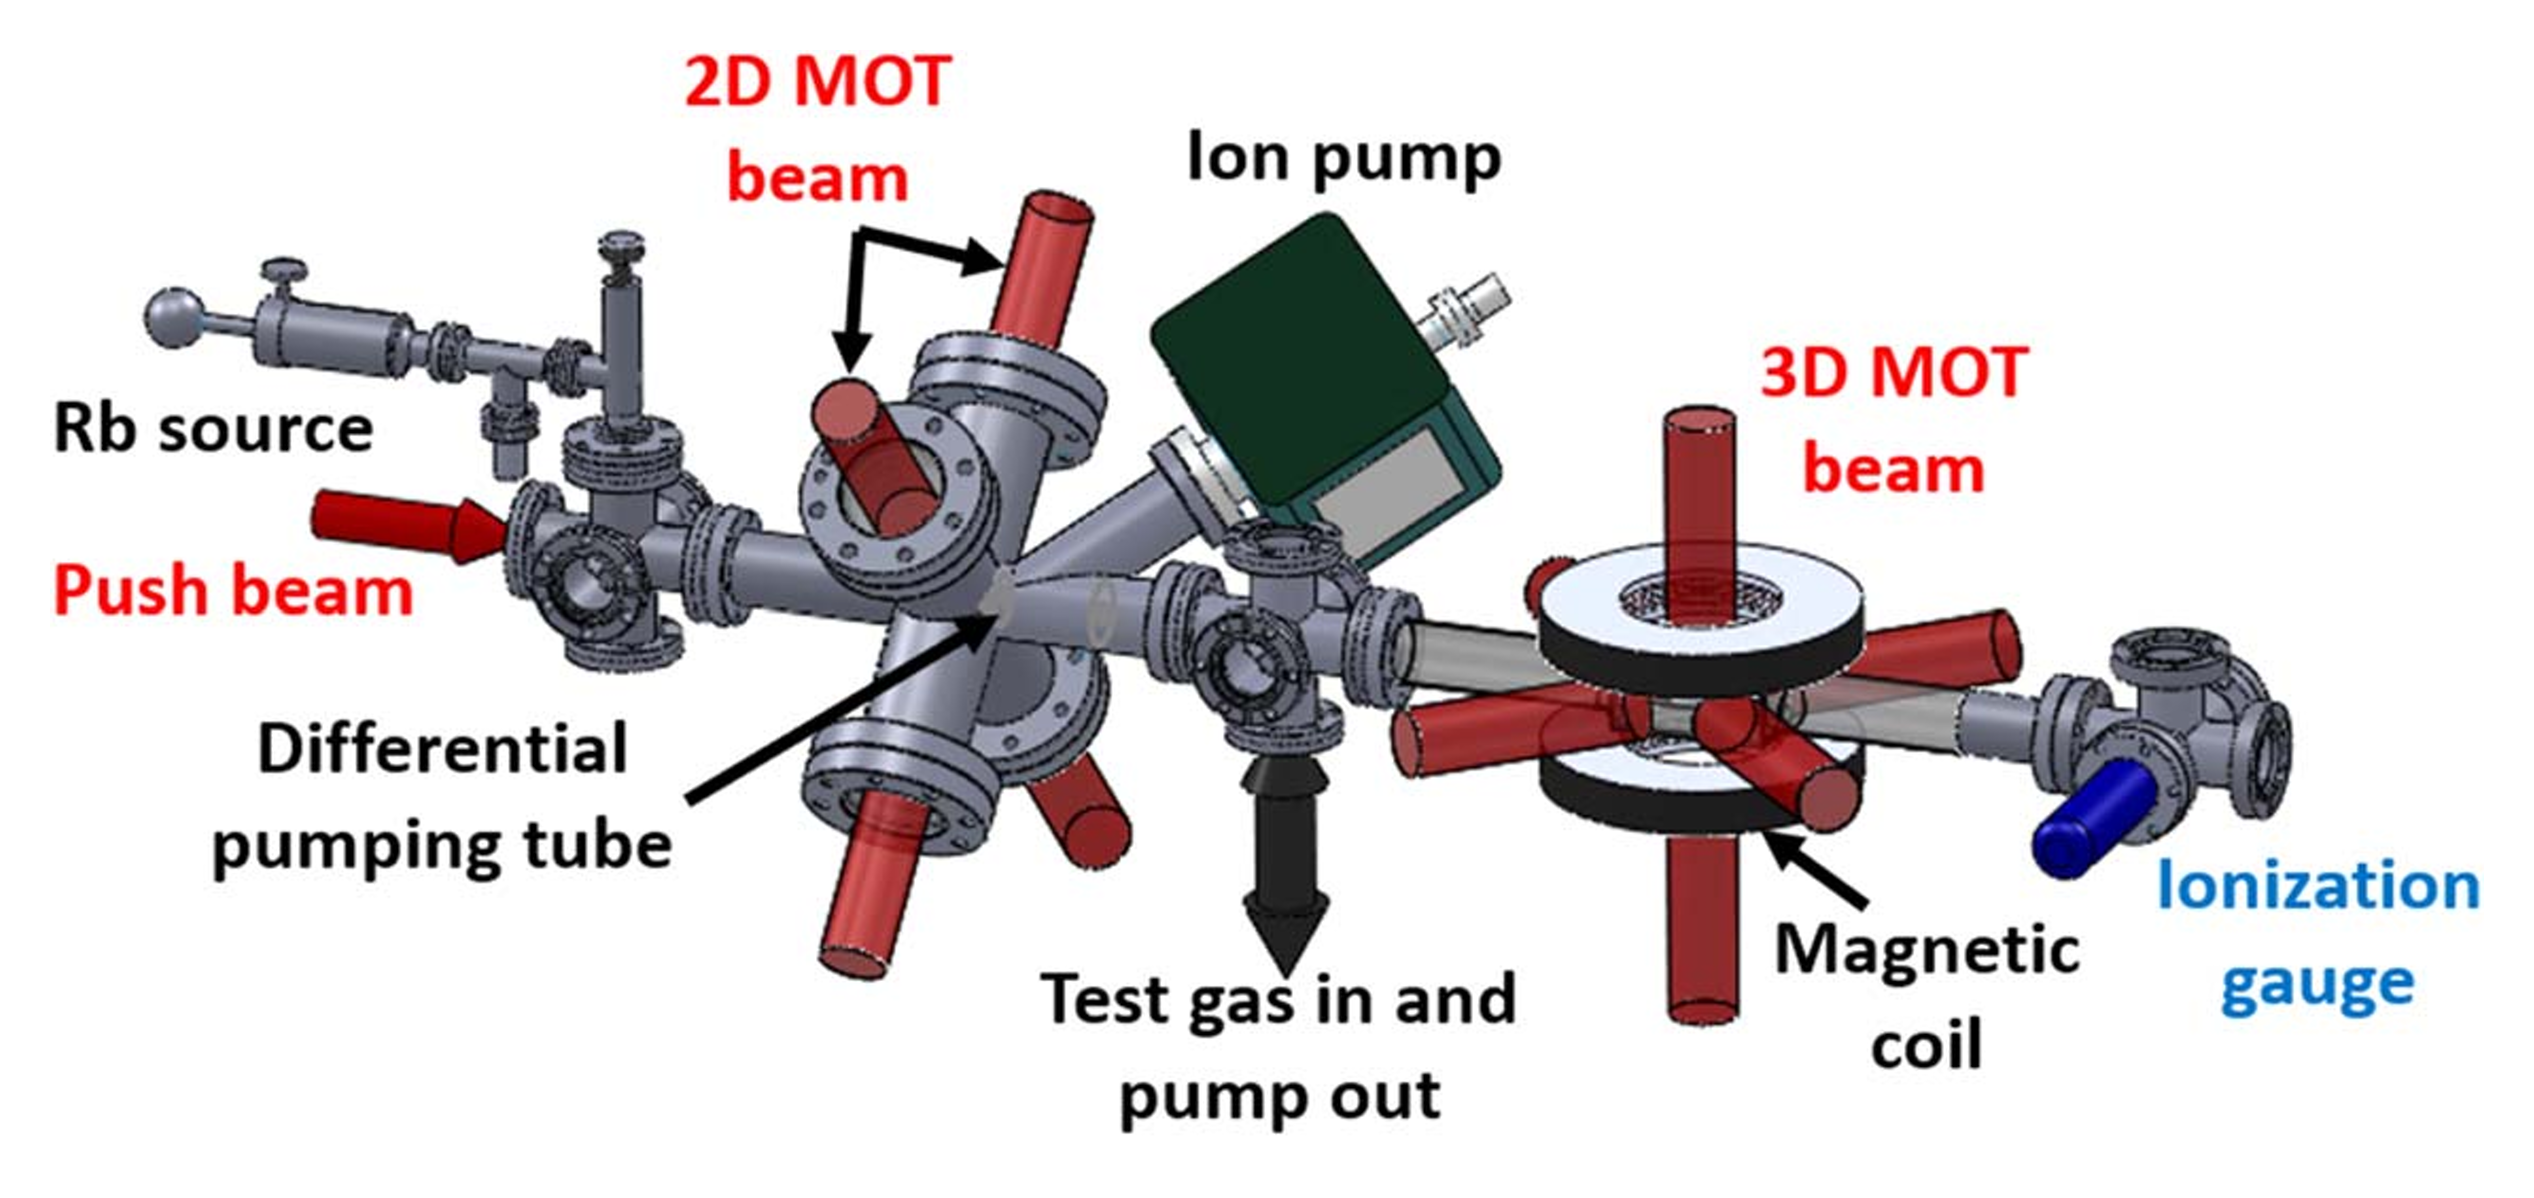
\includegraphics[width=0.6\linewidth]{figs/ch1-3.png} \caption{UBC基于铷原子的量子真空计量方案\cite{boothUniversalityQuantumDiffractive2019}} \label{fig:ch1-3} 
\end{figure}

在国内，冷原子真空计量研究同样发展迅速。以兰州空间技术物理研究所和华东师范大学等单位为代表的研究团队，围绕基于锂冷原子的真空计量方法开展了系统性研究\cite{fengImprovedDesignMagnetic2025,zhangVacuumPressureMeasurement2023,张苏钊基于磁光阱中6Li冷原子的真空度测量2022,成永军基于7Li冷原子操控的超高真空测量2024}，如图\ref{fig:ch1-4}。主要内容包括原子损失率与背景气体压强之间的定量标定、不同气体组分下灵敏度系数的分析以及系统不确定度评估等。在实验实现层面，国内已建立较为成熟的冷原子实验平台并取得阶段性进展，但在装置便携化设计、系统工程化集成以及长期稳定运行能力等方面仍有进一步提升空间。

\begin{figure}[htbp] \centering 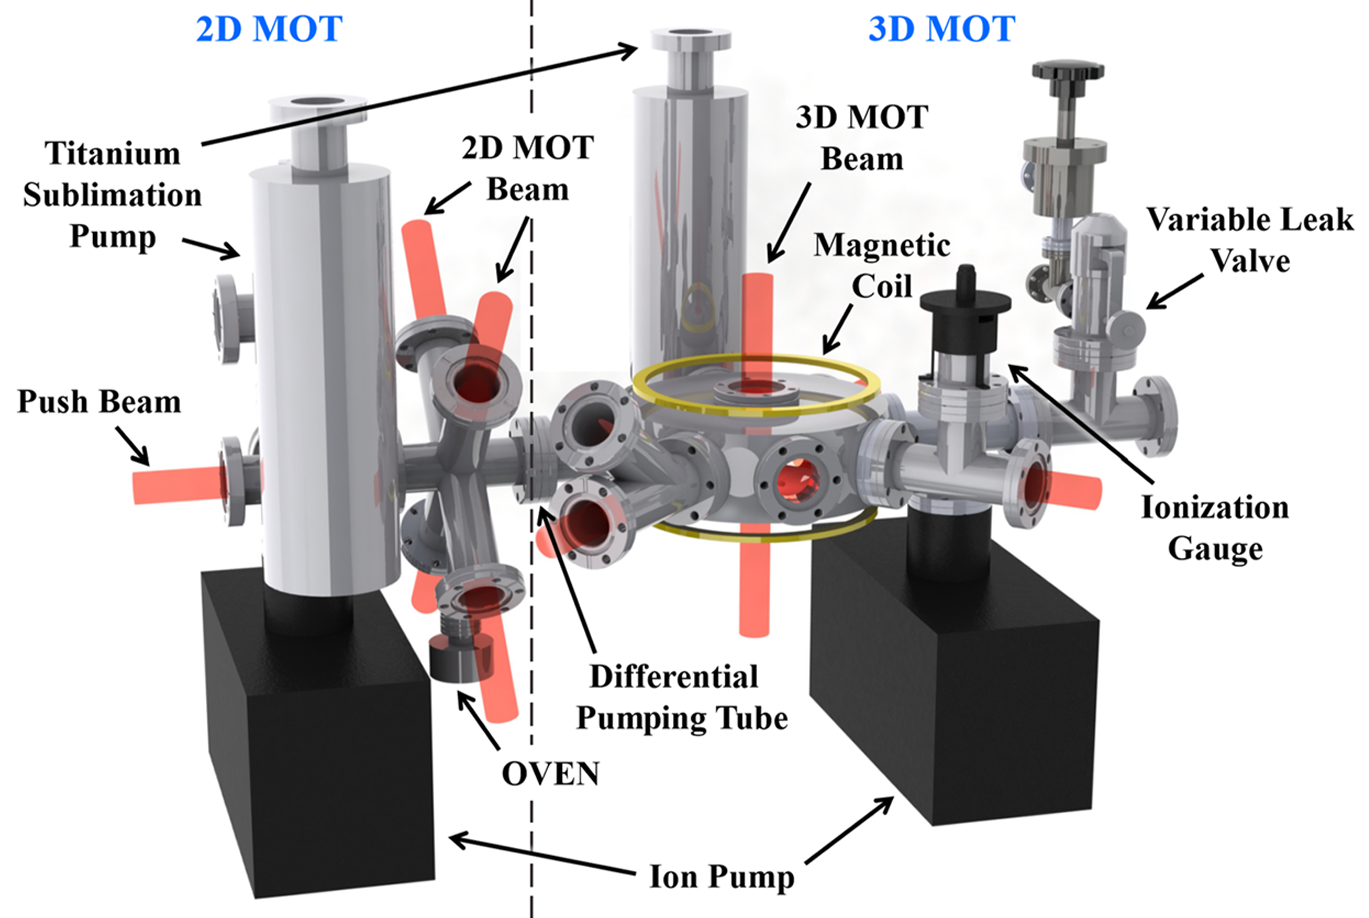
\includegraphics[width=0.6\linewidth]{figs/ch1-4.png} \caption{兰州空间技术物理研究所基于锂原子的实验室级量子真空计量方案\cite{zhangVacuumPressureMeasurement2023}} \label{fig:ch1-4} 
\end{figure}


综上所述，冷原子真空测量技术在物理机理验证与计量模型构建方面已趋于成熟，但在工程化实现与实际应用推广方面仍面临挑战，尤其体现在系统小型化、结构集成度以及长期稳定性等关键指标尚未完全定型。因此，依托中科院精密测量院在冷原子量子技术领域的研究基础，开展面向工程应用的小型化冷原子真空测量装置设计与测试研究，对于提升我国在量子真空计量领域的自主创新能力具有重要意义。

\section{研究内容和论文结构安排}

本课题围绕“小型化冷原子真空计量系统磁光阱装载实验”这一核心目标展开研究。冷原子真空计量技术利用原子与背景气体碰撞导致的损失过程来反演真空压强，其测量结果具有良好的可溯源性与物理可靠性。然而，传统冷原子实验装置通常体积较大、结构复杂，限制了该技术在实际应用场景中的推广。因此，本研究在既有理论模型与实验原理的基础上，重点探索冷原子真空测量系统的小型化实现方案，并通过系统实验对其性能进行验证。

本研究的核心思路是，在保证冷原子俘获与寿命测量条件的前提下，通过系统结构优化与实验流程改进，实现装置的紧凑化设计与稳定运行。与侧重计量标准建立或基本原理验证的研究工作相比，本课题更加关注系统工程实现过程，强调装置结构的可实现性与应用适配能力，从而为冷原子真空测量技术向实际工程应用过渡提供实验依据和技术参考。

在系统设计方面，本研究从光学系统、磁场系统以及真空系统三个方面对实验装置进行了整体优化。

在光学系统设计方面，引入小型化光路技术，对整体光路结构进行紧凑布局设计。通过合理采用分光与合束结构优化光束传输路径，在降低系统空间占用的同时保证光束的准直质量与功率稳定性，从而满足磁光阱对激光参数的要求。

在磁场系统设计方面，本研究采用永磁体与电磁线圈相结合的复合磁场结构，以产生磁光阱与磁阱所需的四极磁场梯度。与传统纯电磁线圈方案相比，该结构能够有效避免水冷系统带来的能耗问题与结构复杂性，从而显著降低系统体积与功率需求。同时，通过磁路设计与磁场分布仿真，对磁场梯度和空间分布进行优化，使其满足原子俘获条件，并兼顾系统调节能力与装配精度要求。

在真空系统设计方面，实验装置在保证小型化结构的同时兼顾光学访问需求。通过合理布置腔体视窗位置与抽气接口，在结构紧凑性与抽气效率之间取得平衡，从而保证系统能够满足冷原子实验所需的超高真空环境。

在系统测试方面，首先开展冷原子磁光阱俘获实验，包括原子云形态观察、荧光信号测量以及俘获原子数估算，以验证实验系统能够稳定实现原子俘获。之后会进行原子寿命测量实验，通过记录磁阱中原子数随时间的衰减曲线提取原子损失率参数，并建立其与背景气体压强之间的关系。最后将测量结果与传统电离规读数进行对比分析，以评估系统测量结果的一致性与重复性。通过多组实验数据的统计分析，对系统可能存在的误差来源进行讨论，并提出相应的改进方案。

通过上述研究工作，本课题完成了从系统设计、实验实现到性能验证的完整研究过程，突出了工程实践特点，为小型化冷原子真空测量系统的进一步发展提供了实验依据与技术参考。

本文的结构安排如下：第一章回顾冷原子真空计量技术的发展历程，总结国内外相关研究进展，并明确本研究的目标与定位。第二章介绍实验装置各组成部分的基本原理与设计方案，包括真空系统、激光系统和磁场系统的具体构建。第三章阐述磁光阱装载实验及实验结果。



	%\chapter{实验装置}

冷原子真空计量实验的成功实现依赖于一套复杂精密的实验平台。该平台的核心在于构建三大子系统：\textbf{超高真空系统}、\textbf{激光冷却系统}以及\textbf{磁场系统}。其中，超高真空环境旨在有效抑制背景气体碰撞，是实现长寿命原子俘获与精确真空计量的物理基础；激光系统主要负责原子的冷却、俘获与量子态制备；磁场系统则用于构建势阱以稳定囚禁原子。

本章将对上述关键子系统进行分模块的详细阐述。首先介绍真空系统的整体结构以及超高真空环境的维持和监测机制，随后讨论激光系统的光路设计，最后对磁场系统进行说明。实验装置主体外观如图\ref{fig:ch2-1}所示。

\begin{figure}[htbp]
	\centering
	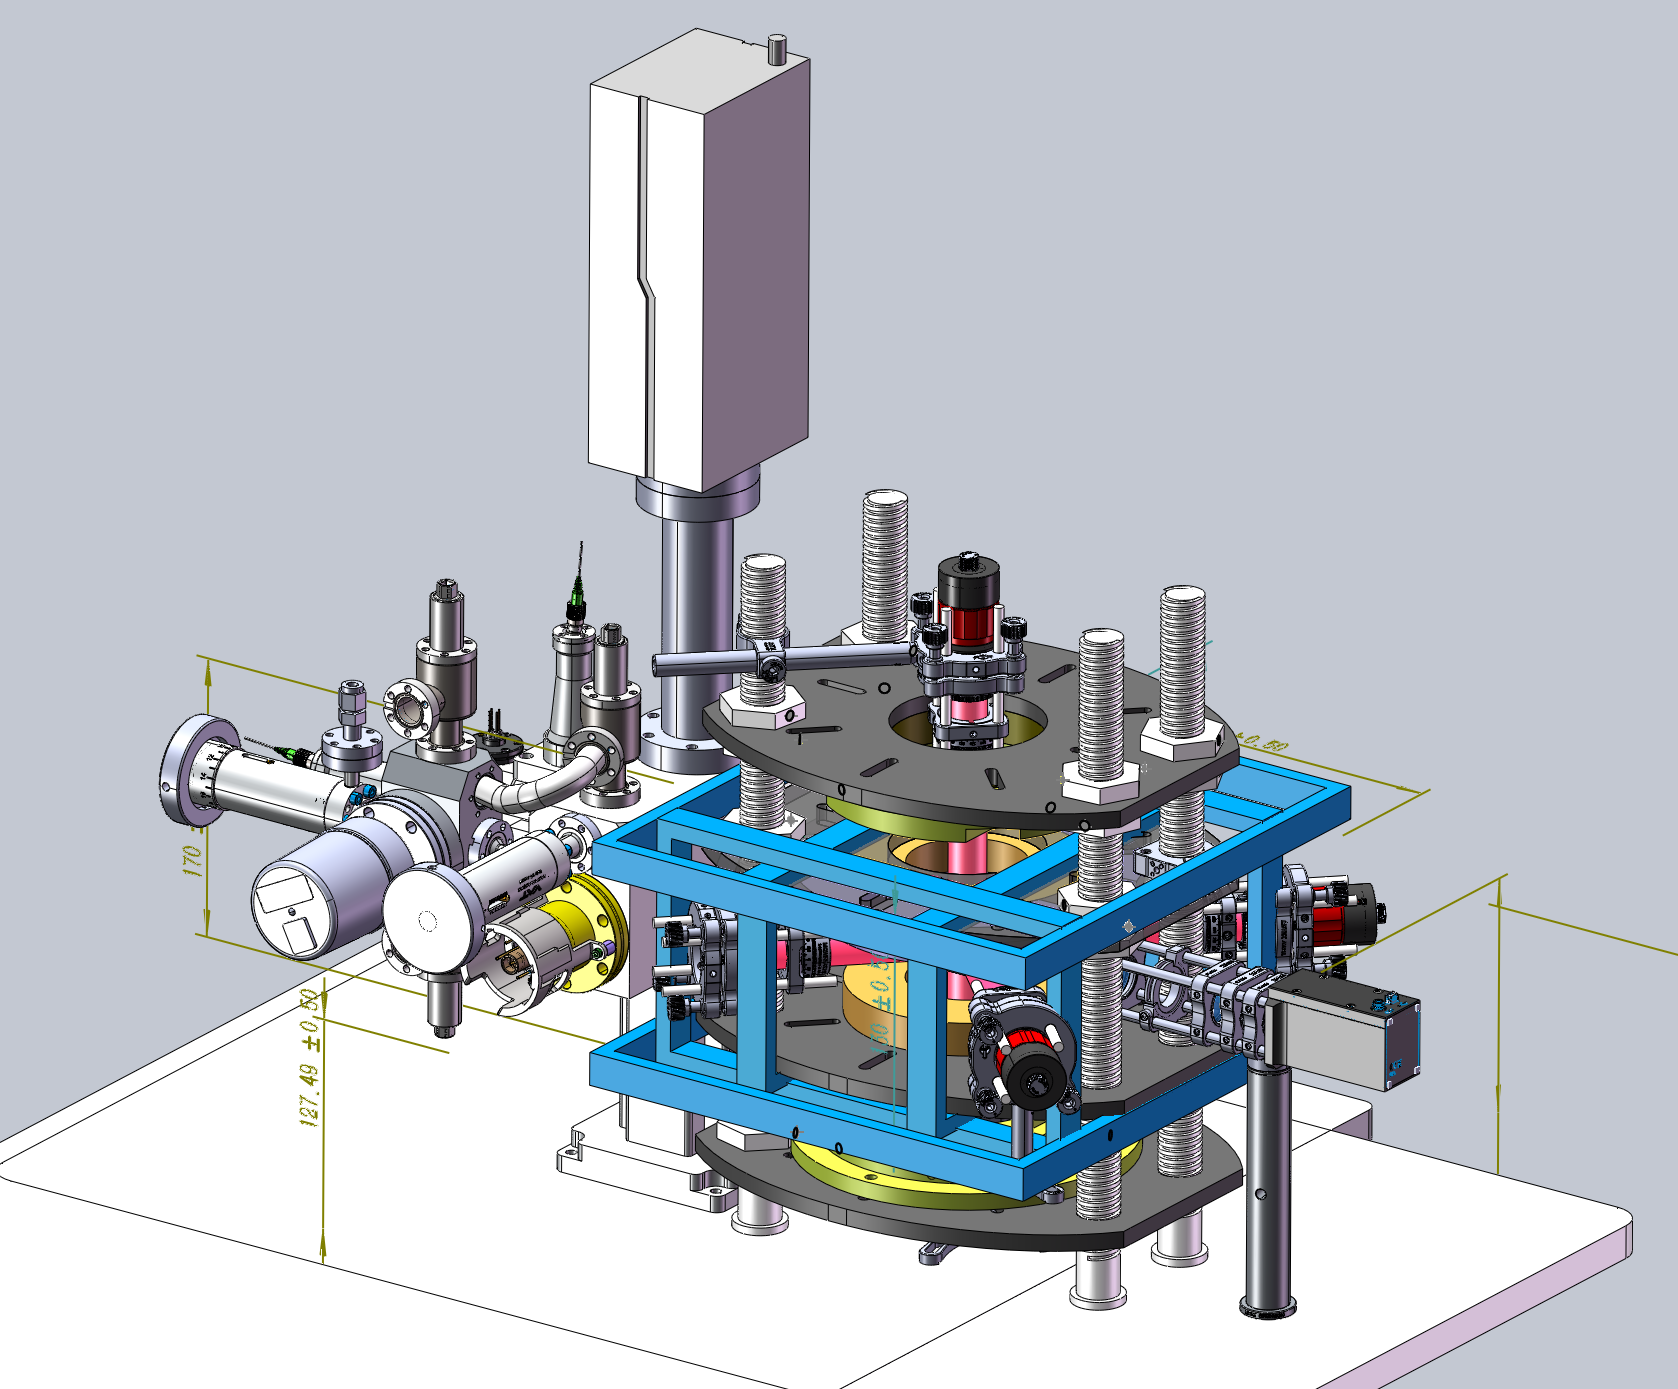
\includegraphics[width=0.6\linewidth]{figs/ch2-1.png}
	\caption{实验装置主体的三维视图}
	\label{fig:ch2-1}
\end{figure}

\section{真空系统}

实现超高真空条件下的精确计量，首要前提是构建一个长期稳定且可控的超高真空环境。本实验所采用的超高真空腔体构成了整个装置的核心平台。本节将从真空系统的机械结构、残余气体成分分析以及真空环境的维持与实时监测三个方面进行详细介绍。

\subsection{真空系统的结构}

真空腔体的整体结构如图\ref{fig:ch2-3}所示，系统由二维磁光阱（Two-dimensional Magneto-optical Trap, 2D MOT）、三维磁光阱（Three-dimensional Magneto-optical Trap, 3D MOT）、复合抽气系统以及真空计量模块等多个功能单元构成。

\begin{figure}[htbp]
	\centering
	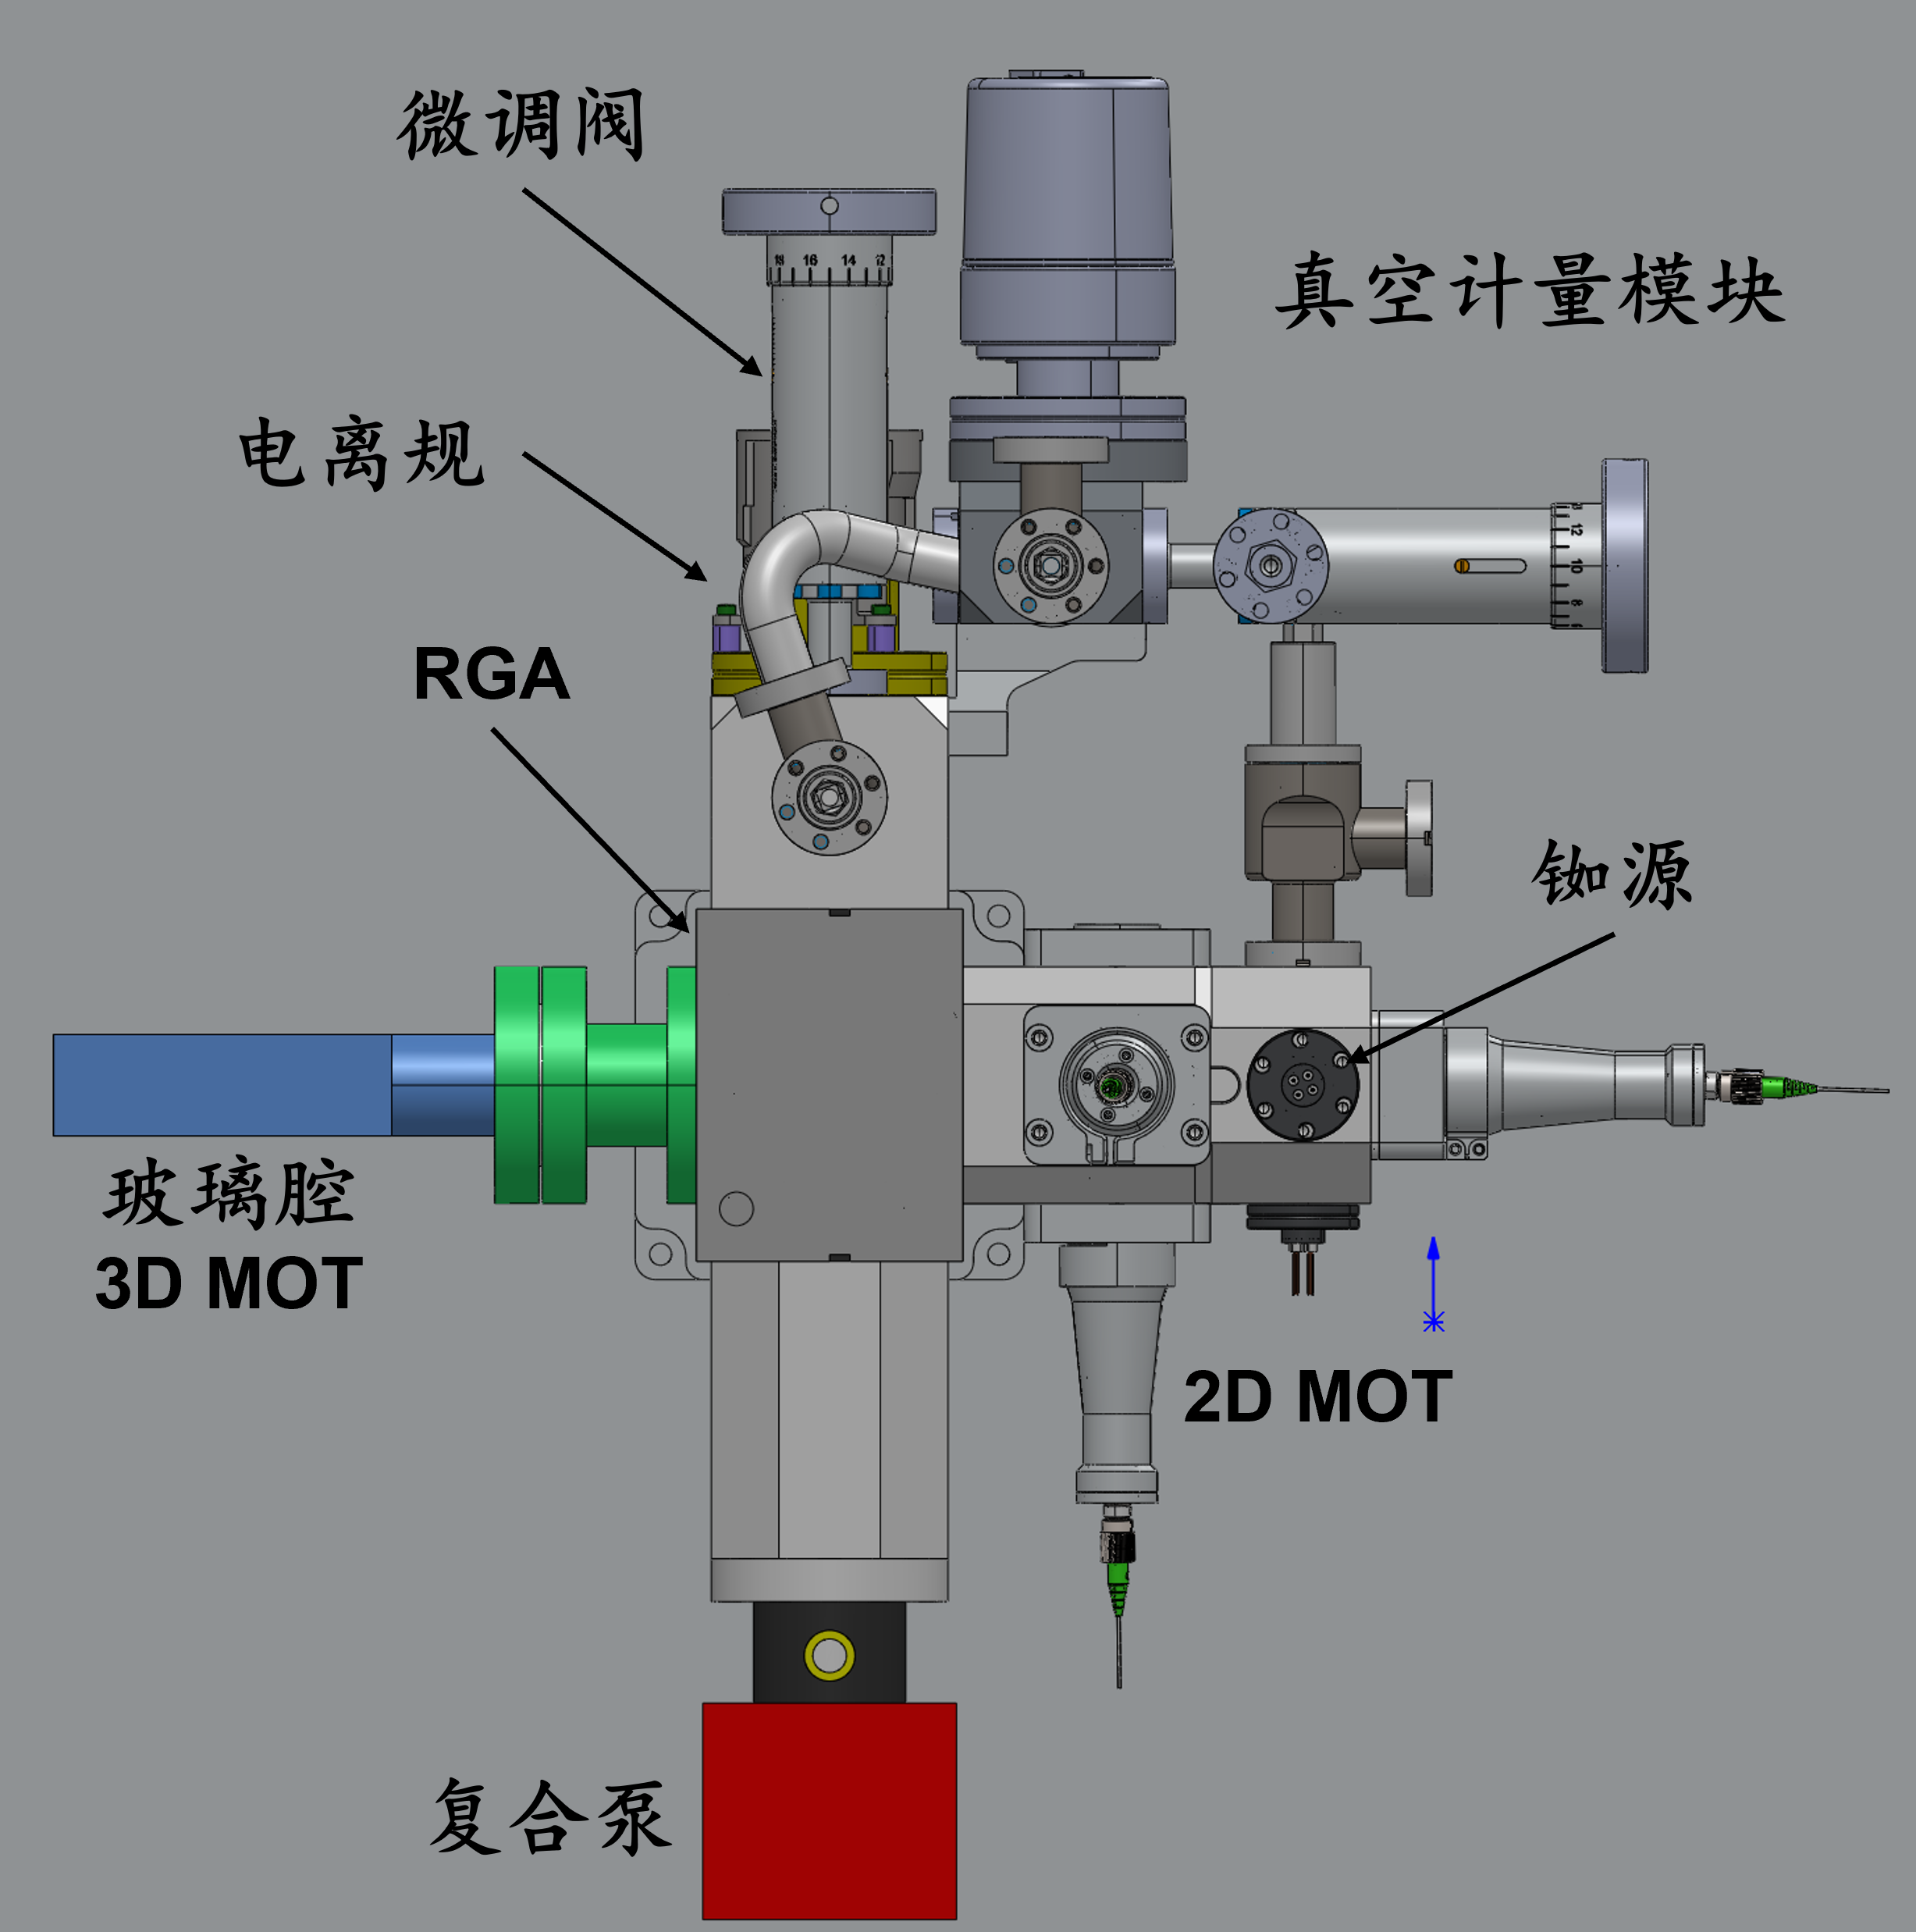
\includegraphics[width=0.6\linewidth]{figs/ch2-3.png}
	\caption{真空系统的俯视图}
	\label{fig:ch2-3}
\end{figure}

2D MOT 区域内部集成有碱金属释放器（dispenser），其内封装高纯度铷源。通过对内置电热丝通电加热，可释放铷蒸气，其中包含自然丰度分布的 $^{85}\mathrm{Rb}$ 与 $^{87}\mathrm{Rb}$ 同位素。实验中可根据需求选择性俘获特定同位素，从而实现不同工作模式的切换。此外，2D MOT 腔体配置有五个高透过率光学窗口，用于引入冷却光与推送光束；窗口外侧环绕安装有磁场线圈，以产生二维磁光阱所需的梯度磁场。

在 2D MOT 区域中，铷原子首先被预冷却并俘获，随后形成具有一定方向性的原子束流，通过差分抽气结构注入至 3D MOT 区域。3D MOT 区域采用镀膜玻璃腔体，并通过法兰与主真空系统连接。由于 2D MOT 需要维持相对较高的铷蒸气分压以提高装载效率，而 3D MOT 对背景气体碰撞极为敏感，因此实验中采用差分管实现两区域的连接与隔离，从而在保证原子通量的同时维持显著的压力梯度，使 3D MOT 区域达到超高真空水平。

为维持系统所需的超高真空环境，真空腔体配备了复合型抽气系统（通常包括离子泵与非蒸发吸气泵），用于持续清除腔体内的残余气体分子，从而保证系统的长期稳定运行。

真空计量模块主要由微调阀、波纹管等气路组件构成，用于实现高纯气体的精确引入。模块中集成高精度电离规，用于实时监测腔体压强，并为冷原子真空计量提供传统测量手段的对照基准。此外，系统顶部还安装有残余气体分析仪（Residual Gas Analyzer, RGA），如图\ref{fig:ch2-1}所示，可对腔体内气体成分及其分压进行定量分析。

\subsection{真空系统中残余气体成分分析}

在小型化冷原子真空计量系统中，不同背景气体分子与铷原子之间的碰撞截面存在显著差异，从而直接影响基于原子损失率的压强反演结果。因此，在实验开展之前，有必要对真空腔体内残余气体的组分及其分压进行定量分析，以确定适用于压强反演计算的有效碰撞截面参数。

本实验采用美国斯坦福研究系统（Stanford Research Systems, SRS）RGA100 残余气体分析仪（Residual Gas Analyzer, RGA），如图\ref{fig:ch2-6}所示。该设备可在 $1 \sim 100~\mathrm{amu}$ 的质量范围内对气体组分进行分辨，并实现各组分分压的定量测量\cite{ResidualGasAnalyzer}，为后续冷原子真空计量中的压强反演提供关键实验依据。

\begin{figure}[htbp]
	\centering
	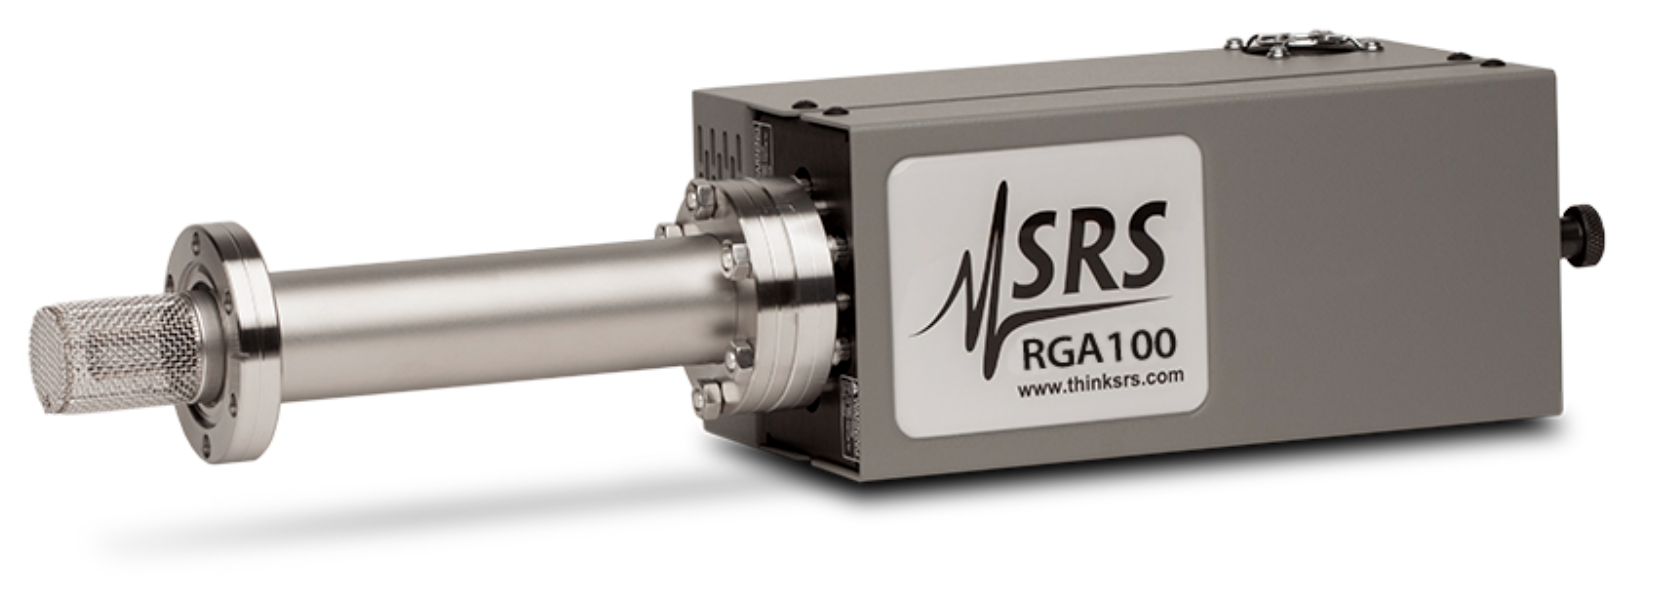
\includegraphics[width=0.6\linewidth]{figs/ch2-6.png}
	\caption{RGA100 残余气体分析仪实物图\cite{ResidualGasAnalyzer}}
	\label{fig:ch2-6}
\end{figure}

除实验过程中人为引入的高纯气体外，真空系统中还存在多种不可避免的残余气体来源。图\ref{fig:ch2-7}给出了在未通入外界气体条件下腔体内残余气体的组分分布。

\begin{figure}[htbp]
	\centering
	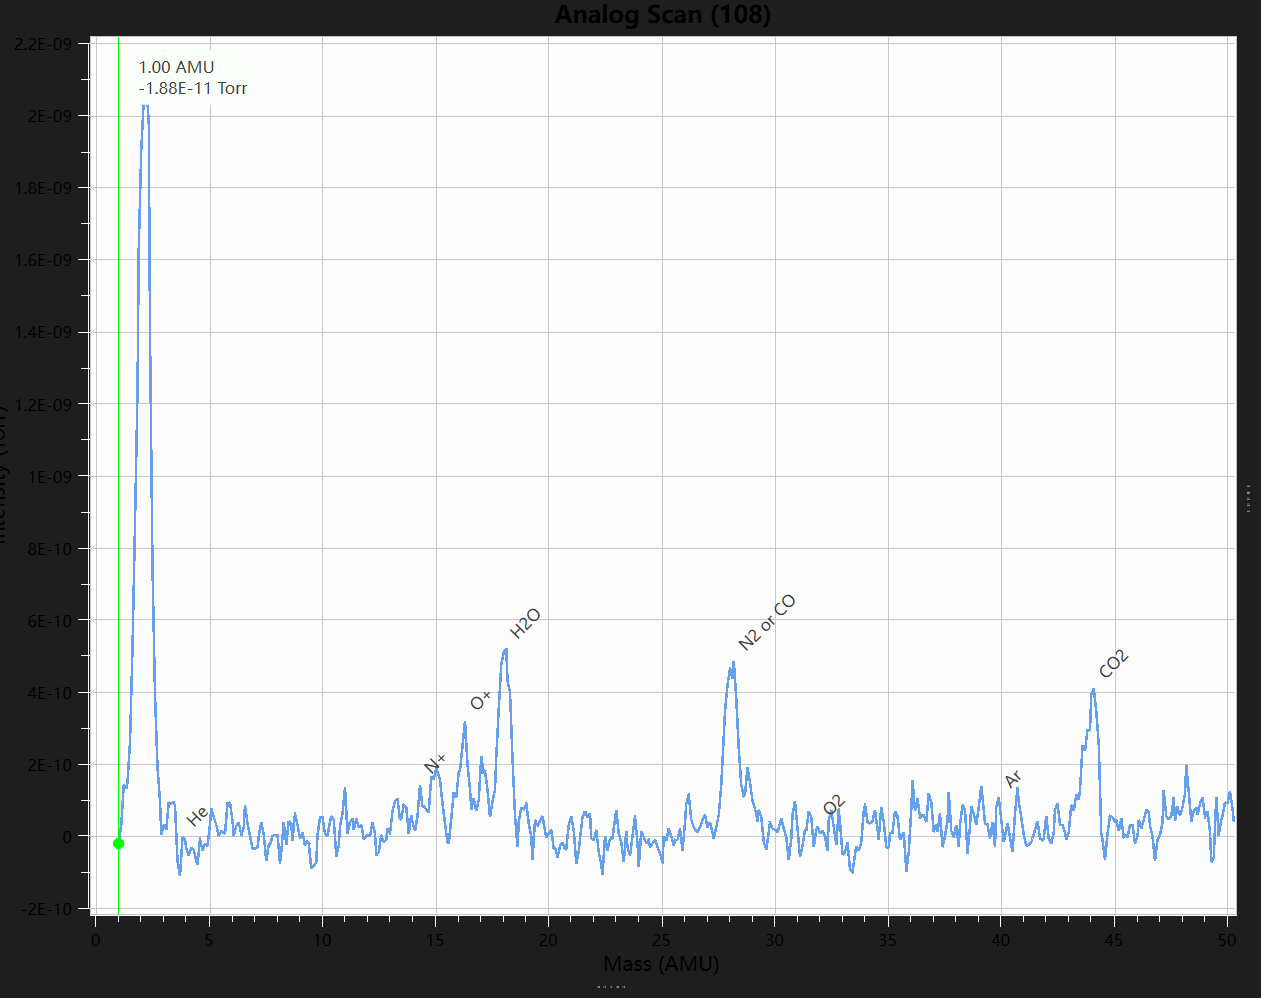
\includegraphics[width=0.6\linewidth]{figs/ch2-7.png}
	\caption{未通入外界气体时真空腔中残余气体的组分分布情况}
	\label{fig:ch2-7}
\end{figure}

首先，真空系统的泄漏是气体载入的重要来源之一。需要指出的是，“绝对无泄漏”的真空系统在实际中难以实现，工程上只能将泄漏控制在可忽略水平。常见泄漏位置包括 CF 法兰密封面、焊接接缝以及波纹管等结构薄弱区域。真实泄漏的一个典型特征是其残余气体组分比例与标准大气成分相近（例如 $\mathrm{N}_2$ 与 $\mathrm{O}_2$ 占主导）。然而，从图\ref{fig:ch2-7}可以看出，本系统中氢气占据主导地位，说明外界泄漏对气体本底的贡献较小，系统整体密封性能良好。

当系统经过充分抽气与烘烤处理后，材料本底出气成为限制极限真空度的主要因素。所谓材料出气，是指真空系统中结构材料及功能元件（如电离规灯丝、RGA 灯丝等）表面吸附或体相中溶解的气体，在真空环境下通过表面解吸或体扩散机制释放进入腔体的过程。本实验系统的主要材料包括不锈钢、玻璃以及无氧铜。在室温条件下，其主要出气组分为质量数为 $18~\mathrm{amu}$ 的水蒸气（$\mathrm{H}_2\mathrm{O}$）以及 $2~\mathrm{amu}$ 的氢气（$\mathrm{H}_2$）。

针对不同来源的气体，需要采用相应的烘烤除气策略。水蒸气主要来源于材料表面的物理吸附层，其去除依赖于中温烘烤（约 $150 \sim 200^\circ\mathrm{C}$），通过加速表面解吸过程可显著降低其分压；而氢气则主要来源于不锈钢材料体相中溶解的氢原子，其去除依赖于高温烘烤（通常 $\sim 300^\circ\mathrm{C}$），以促进氢在材料内部的扩散并逸出至真空环境中。经过长时间烘烤除气处理后，系统中水蒸气分压显著降低，而氢气逐渐成为超高真空环境中的主导气体组分，如图\ref{fig:ch2-7}所示。

最终，系统可稳定达到 $10^{-9}~\mathrm{Pa}$ 量级的超高真空水平，为冷原子体系的长寿命俘获及高精度真空计量提供必要条件。


\subsection{真空环境的维持与实时监测}

本实验中的超高真空环境由意大利 SAES Getters 公司研制的 NEXTorr\textsuperscript{\textregistered} Z200 一体化复合型超高真空泵维持。该装置将\textit{非蒸散型吸气剂（Non-Evaporable Getter, NEG）模块}与\textit{溅射离子泵（Sputter Ion Pump, SIP）模块}高度集成于标准全金属 ConFlat（CF）法兰结构中，实现了无油、无机械振动、无噪声的长期稳定运行，同时其内部无任何运动部件，具有极高的可靠性与运行寿命。

其中，NEG 模块采用 SAES 专利的 ZAO\textsuperscript{\textregistered}（Zr–V–Ti–Al）多孔烧结合金材料，能够通过化学吸附机制高效捕获活性气体分子。针对超高真空系统中占主导地位的氢气（\ce{H_2}），其峰值抽速可达 \SI{290}{\liter\per\second}，总吸气容量约为 \SI{1160}{torr\cdot\liter}。该泵的极限真空度优于 \SI{1e-11}{mbar}。此外，设备在结构设计上进行了低磁场优化，在距离泵体 \SI{10}{\centi\meter} 处的杂散磁场强度低于 \SI{1}{\micro\tesla}，从而有效避免对磁光阱（MOT）所需高均匀度磁场分布的扰动\cite{NEXTorrUHVPumps}。

NEG 与 SIP 模块的协同工作实现了对不同气体组分的互补抽气。具体而言，NEG 模块主要负责抽除活性气体（如 \ce{H_2}、\ce{CO}、\ce{N_2}、\ce{H_2O} 等），而 SIP 模块则用于抽除 NEG 难以有效捕获的惰性气体（如 He、Ar）。这种复合抽气机制能够在长时间尺度上稳定维持腔体内的超高真空环境，从而显著降低背景气体与冷原子的碰撞概率，延长原子俘获寿命，并提高冷原子真空计量的测量精度。

\begin{figure}[htbp]
	\centering
	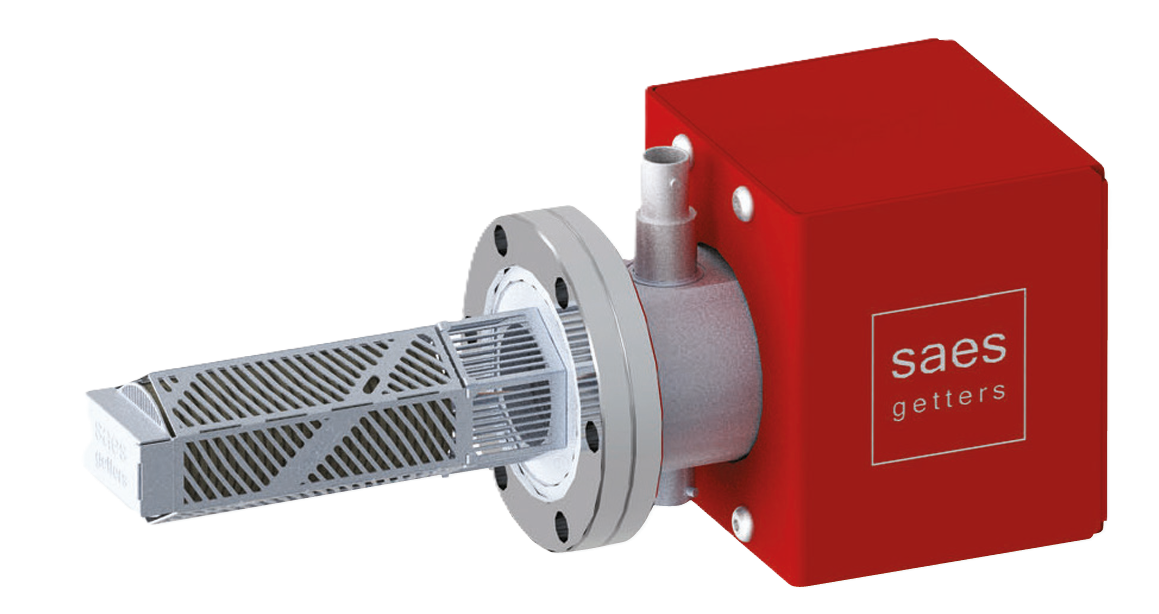
\includegraphics[width=0.6\linewidth]{figs/ch2-4.png}
	\caption{SAES Getters 公司生产的 NEXTorr\textsuperscript{\textregistered} Z200 一体化复合型超高真空泵\cite{NEXTorrUHVPumps}}
	\label{fig:ch2-4}
\end{figure}

在真空度的实时监测方面，本实验采用德国 Leybold 公司 COMBIVAC CM 52 真空控制器配合 IONIVAC IE 514 热阴极电离规，对主腔体压强进行连续测量。电离规基于气体分子在电子轰击下发生电离的原理，通过测量离子电流并结合其与气体数密度之间的近似线性关系，实现对真空压强的反演测量。该设备的测量范围覆盖 \(2 \times 10^{-12} \sim 1 \times 10^{-2}\ \text{mbar}\)，能够满足超高真空区间内高灵敏度与长时间稳定监测的需求\cite{COMBIVACCMPassive}。


\begin{figure}[htbp]
	\centering
	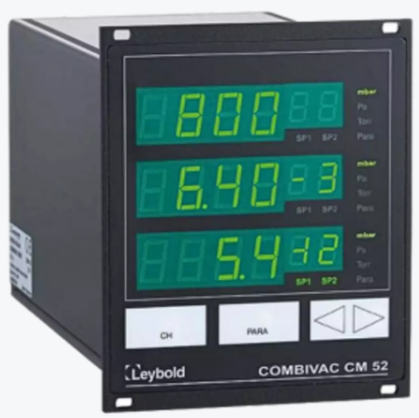
\includegraphics[width=0.3\linewidth]{figs/ch2-5.png}
	\caption{COMBIVAC CM 52 真空控制器\cite{COMBIVACCMPassive}}
	\label{fig:ch2-5}
\end{figure}

\section{激光系统}
\subsection{铷-87原子跃迁谱线}
激光冷却需要一个闭合的循环，但是很难保证准确的跃迁。加上一个泵浦光将暗态抽运回来，如图\ref{fig:ch2-11}。
\begin{figure}[htbp]
	\centering
	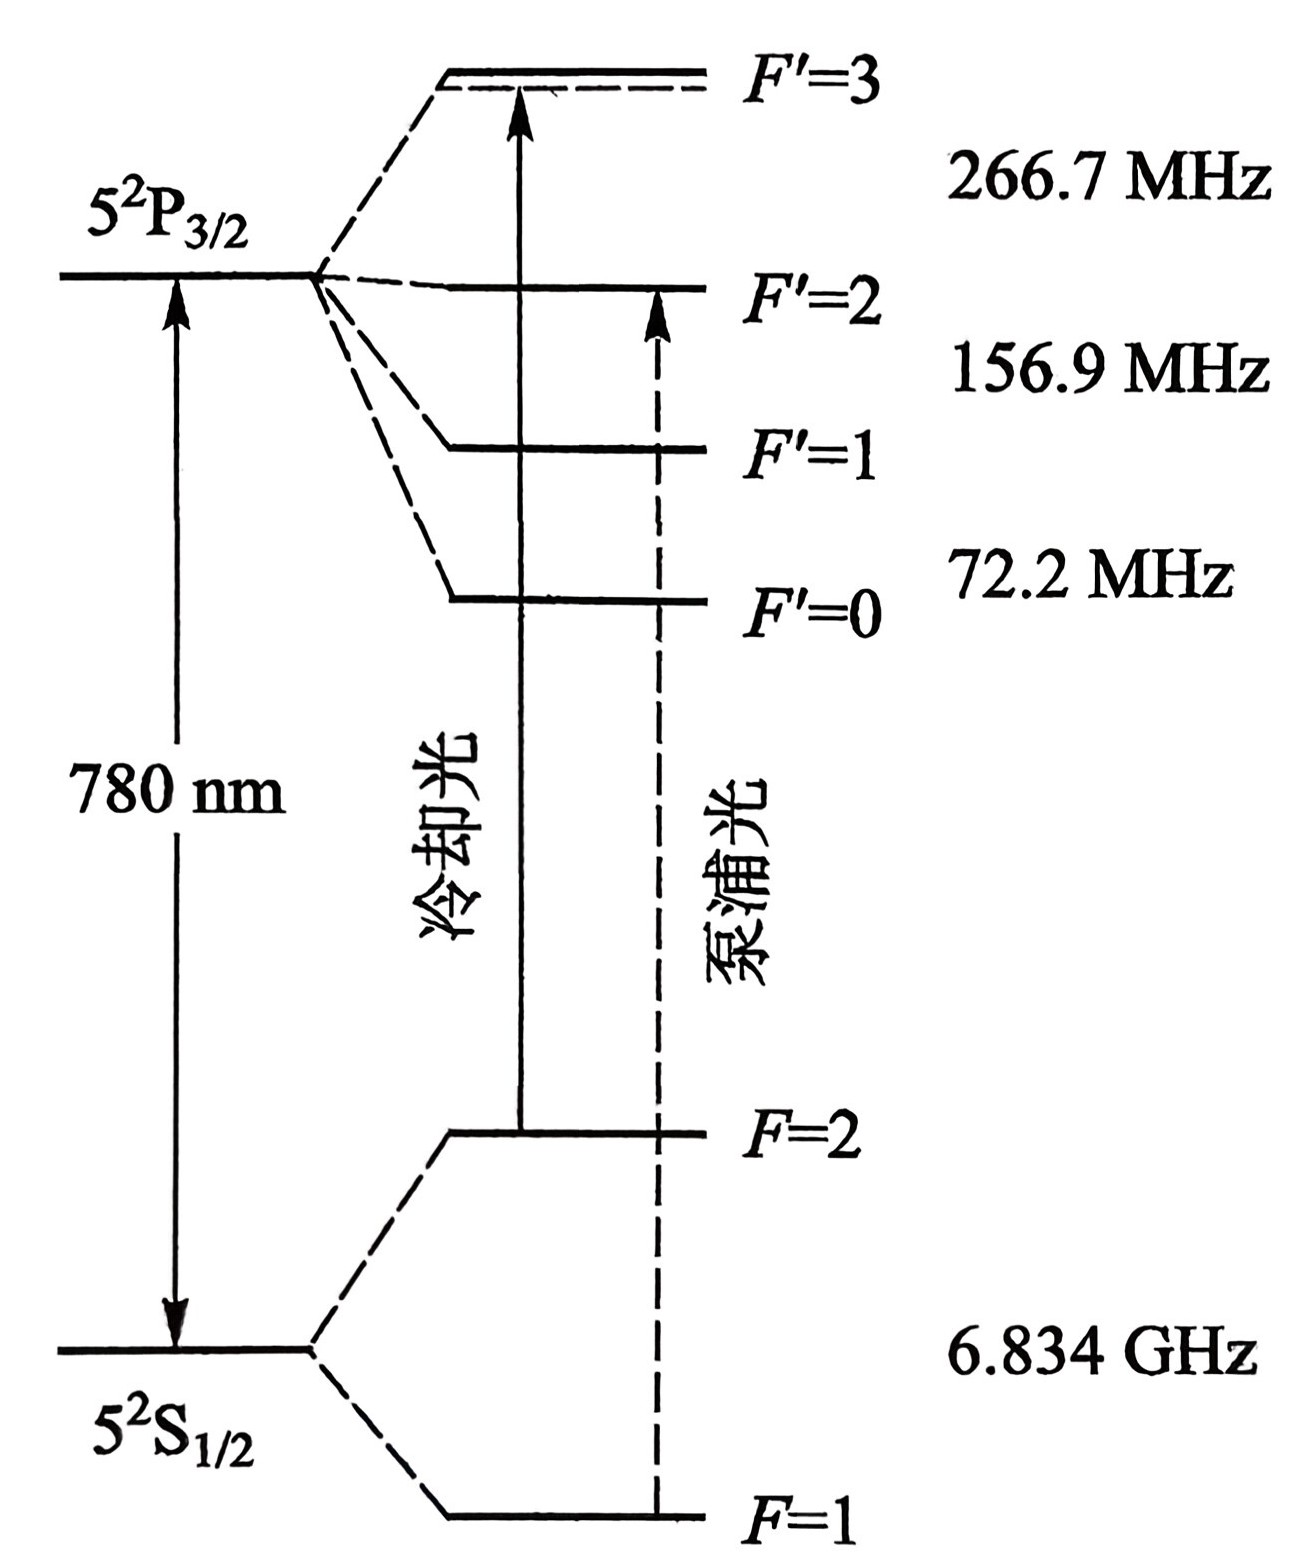
\includegraphics[width=0.4\linewidth]{figs/ch2-11.jpg}
	\caption{铷-87原子跃迁谱线}
	\label{fig:ch2-11}
\end{figure}
\subsection{光路设计}
\section{磁场系统}
\begin{figure}[htbp]
	\centering
	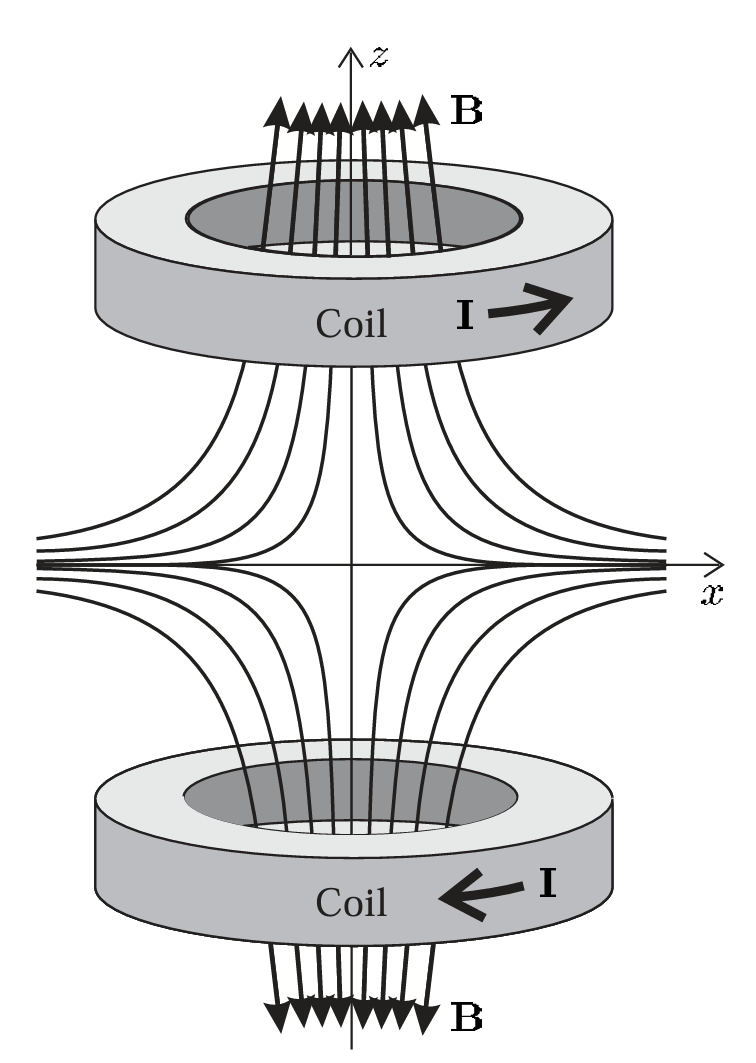
\includegraphics[width=0.4\linewidth]{figs/ch2-10.png}
	\caption{四极磁场}
	\label{fig:ch2-10}
\end{figure}
\begin{figure}[htbp]
	\centering
	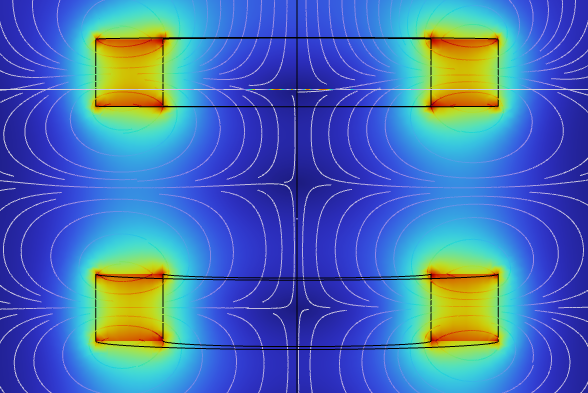
\includegraphics[width=0.5\linewidth]{figs/ch2-12.png}
	\caption{磁场模拟}
	\label{fig:ch2-12}
\end{figure}
	%\chapter{磁光阱装载实验}
本章将重点介绍磁光阱装载实验。激光冷却作为自20世纪80年代发展起来的一项核心冷原子实验技术，为冷原子物理研究提供了关键支撑。本实验采用二维磁光阱（2D MOT）对原子束流进行预冷却处理，随后通过差分管将预冷却后的原子束流送入三维磁光阱（3D MOT）中，最终形成稳定的冷原子团，为后续磁阱装载实验奠定基础。本章将首先系统阐述激光冷却与磁光阱的相关基本原理，随后呈现磁光阱装载的实验结果，并对实验现象及结果进行详细分析与讨论。
\section{激光冷却原理}
激光冷却主要利用光对原子的散射力效应。当静止原子吸收$N$个共振光子后，会通过自发辐射释放这些光子，由于自发辐射具有各向同性，其引起的动量变化相互抵消为零；根据动量守恒定律，原子在吸收光子时会获得相应的反冲动量。考虑到原子本身具有一定的运动速度，会产生多普勒效应，运动原子所观测到的激光频率相较于激光本征频率会发生偏移，当原子与激光相向运动时，需采用红失谐激光方可实现原子与光子的共振相互作用。在小速度近似范围内，原子将受到与运动方向相反、大小正比于速度的阻尼力，进而能够在对射激光场中实现冷却。
\begin{figure}[htbp]
	\centering
	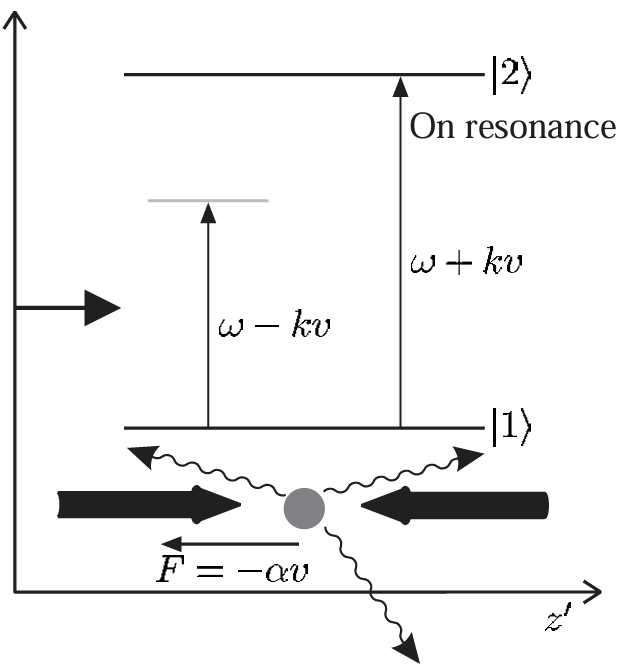
\includegraphics[width=0.4\linewidth]{figs/ch3-1.png}
	\caption{激光冷却原理图}
	\label{fig:ch3-1}
\end{figure}
随机行走计算
\begin{figure}[htbp]
	\centering
	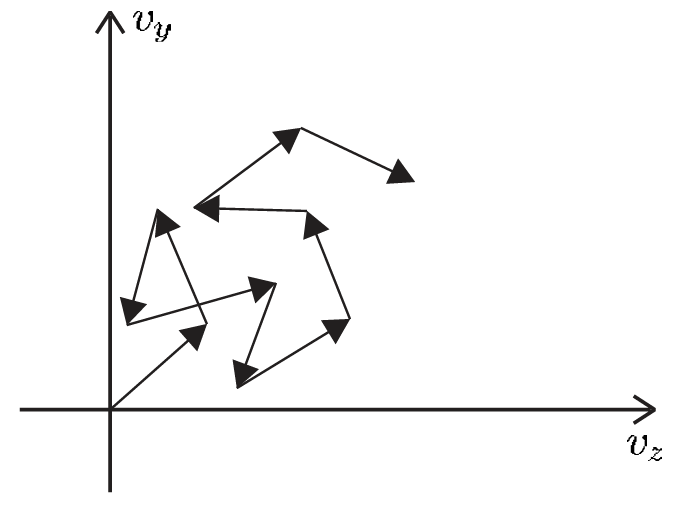
\includegraphics[width=0.4\linewidth]{figs/ch3-2.png}
	\caption{原子在光学黏团中的随机行走}
	\label{fig:ch3-2}
\end{figure}

\section{磁光阱原理}
\begin{figure}[htbp]
	\centering
	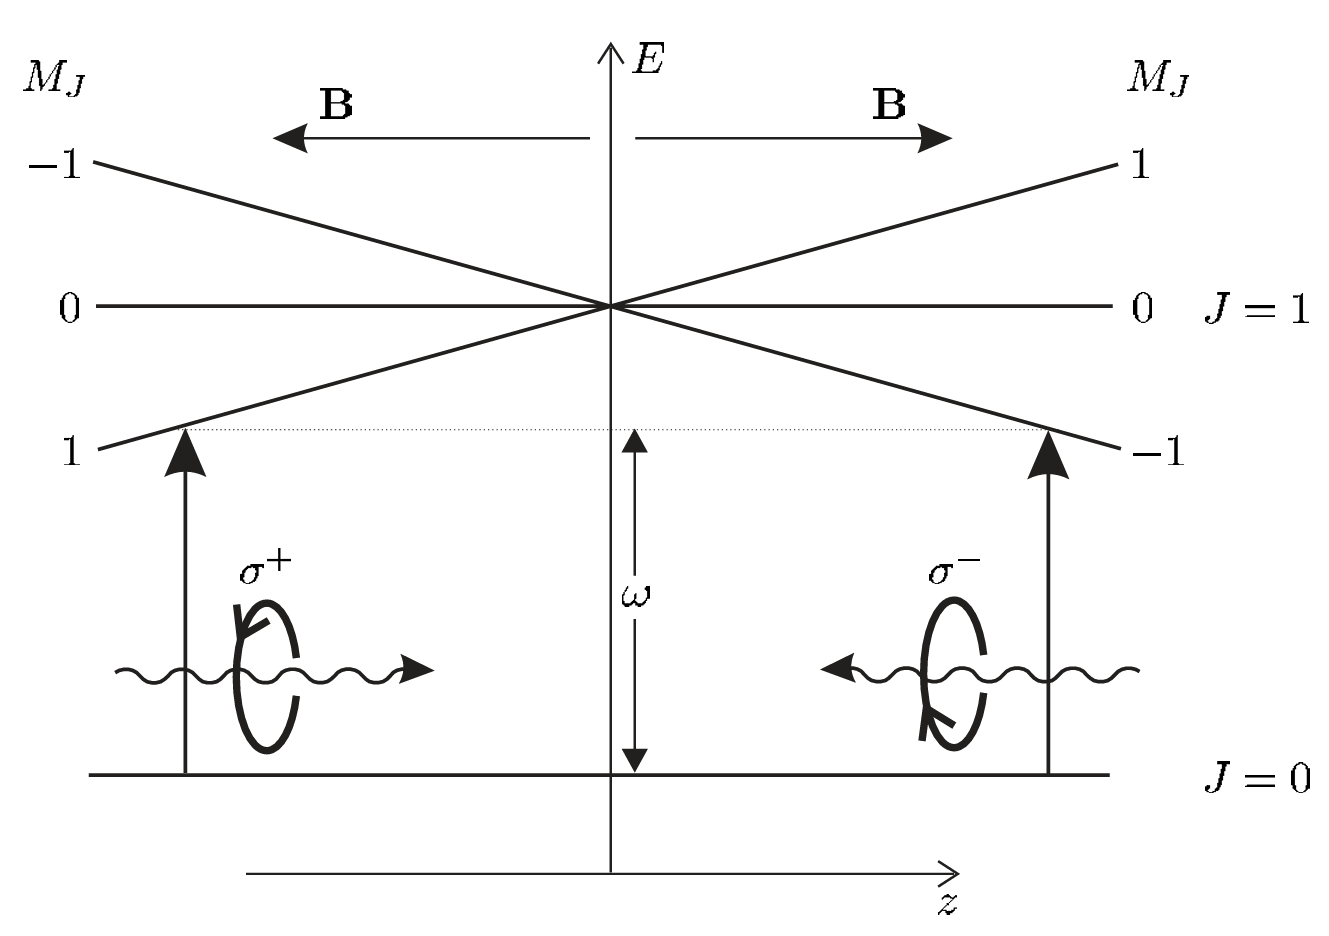
\includegraphics[width=0.4\linewidth]{figs/ch2-8.png}
	\caption{磁光阱原理图}
	\label{fig:ch2-8}
\end{figure}
\begin{figure}[htbp]
	\centering
	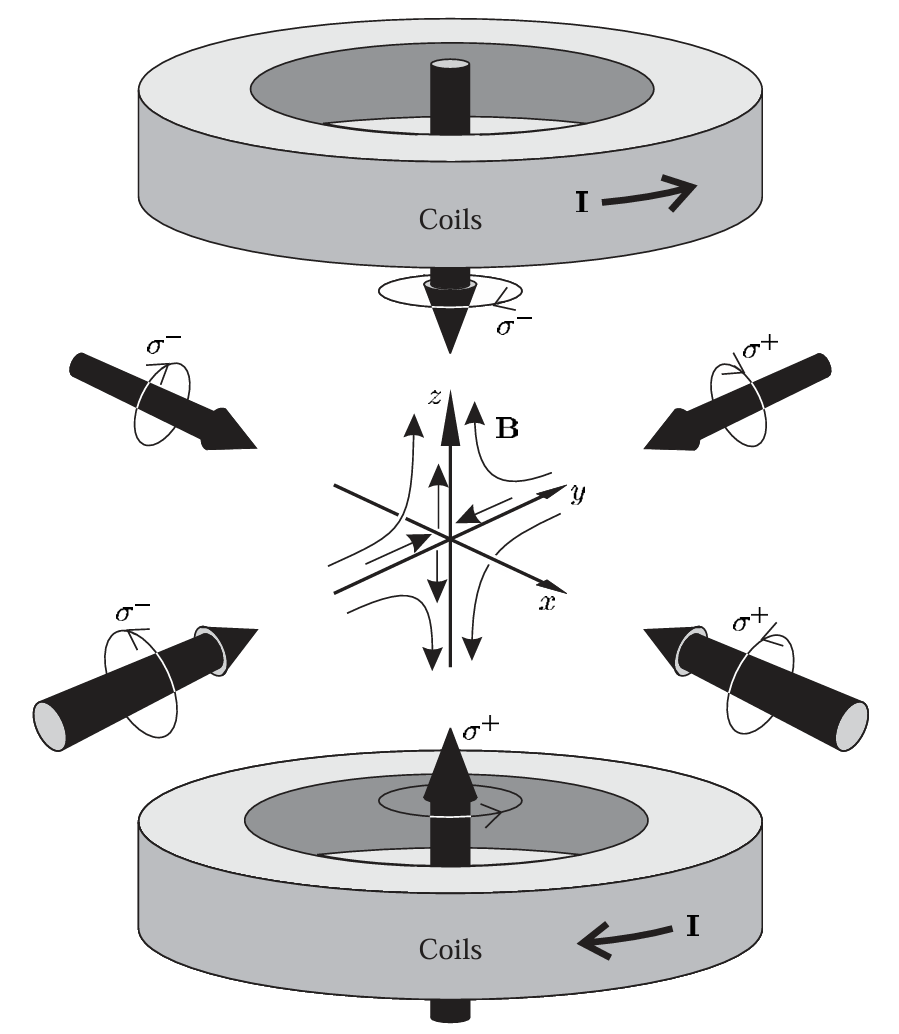
\includegraphics[width=0.4\linewidth]{figs/ch2-9.png}
	\caption{三维磁光阱立体图}
	\label{fig:ch2-9}
\end{figure}
	% 参考文献
	% 参考文献
	\bibliography{ref/CAVS}
	
	
	% 致谢
	%\include{pages/acknowledgement}
	
	% 附录
	\appendix
	%\chapter{原子结构的描述}


在物理学中，处理复杂体系时，我们通常采用\textbf{按能量尺度逐级展开}的方法。这意味着，我们首先找出主导的相互作用项，然后再逐步引入较小的修正项。这种“分层近似”的思想，在原子结构理论中尤为常见。其实，原子哈密顿量在严格的形式下非常复杂，几乎不可能进行高精度计算，所以我们只能依赖实验来获取能级信息。因此，在实际处理中，我们需要对各相互作用的能量量级进行比较，判断哪些项是主导因素，哪些项可以视作微扰修正。这样，我们就能在实验精度的范围内较好地理解原子的行为。

以铷-87（$^{87}\text{Rb}$）原子的能级图为例，AMO实验的第一步就是搞懂这张图\ref{fig:appA-1}。

\begin{figure}[htbp]
	\centering
	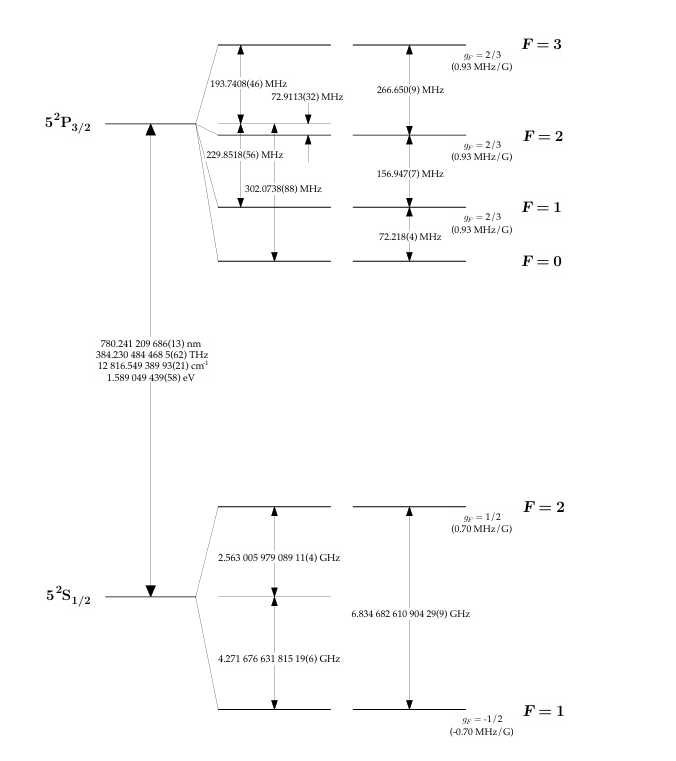
\includegraphics[width=0.6\linewidth]{figs/appB-1.png}
	\caption{铷-87（$^{87}\text{Rb}$）原子的D2线能级图}
	\label{fig:appA-1}
\end{figure}

原子哈密顿量一般可以写作：

\[
\hat{H} = \hat{H}_0 + \hat{H}_\text{SOC} + \hat{H}_\text{HFS} + \hat{H}_B,
\]

其中 $\hat{H}_0$ 是中心场近似下的主哈密顿量，$\hat{H}_\text{SOC}$ 是自旋—轨道耦合项，$\hat{H}_\text{HFS}$ 是超精细相互作用项，$\hat{H}_B$ 是外磁场相互作用项。不同项代表着不同的能量尺度，原子的能级结构正是通过逐步引入这些尺度而形成的。

如果不考虑外场作用，能量尺度最大的是 $\hat{H}_0$。以氢原子为例，当只考虑 $\hat{H}_0$ 时，能级只与主量子数 $n$ 有关。此时，$n,l,m_l$（以及电子自旋量子数 $s,m_s$）都是好量子数，其本征方程是：

\[
\hat{H}_0 \ket{n,l,m_l} = E_n \ket{n,l,m_l},
\]

\[
\hat{L}^2 \ket{n,l,m_l} = l(l+1)\hbar^2 \ket{n,l,m_l},
\]

\[
\hat{L}_z \ket{n,l,m_l} = m_l \hbar \ket{n,l,m_l}.
\]

由于库仑势的对称性，氢原子能级有很高的简并性，正是这种简并形成了我们熟悉的玻尔能级结构。氢原子基态的能量约为 $-13.6\ \text{eV}$，与第一激发态之间的能量差大约是几个eV。

我们研究的主要对象是碱金属原子。原子核与内层电子可等效成一个原子实，价电子与原子实的库仑相互作用构成能量的主项，其能级可表示为
\[
E_{nl} = - R_\infty h c \cdot \frac{1}{(n - \delta_{nl})^2},
\]
其中 $n$ 为主量子数，$\delta_{nl}$ 为量子数亏损。内层电子的存在屏蔽了一部分原子核的正电荷，使有效电荷趋近于1。角量子数 $l$ 越大，电子离原子实越远，屏蔽效果越好，故 $\delta_{nl}$ 越小，如图\ref{fig:appA-2}。
\begin{figure}[htbp]
	\centering
	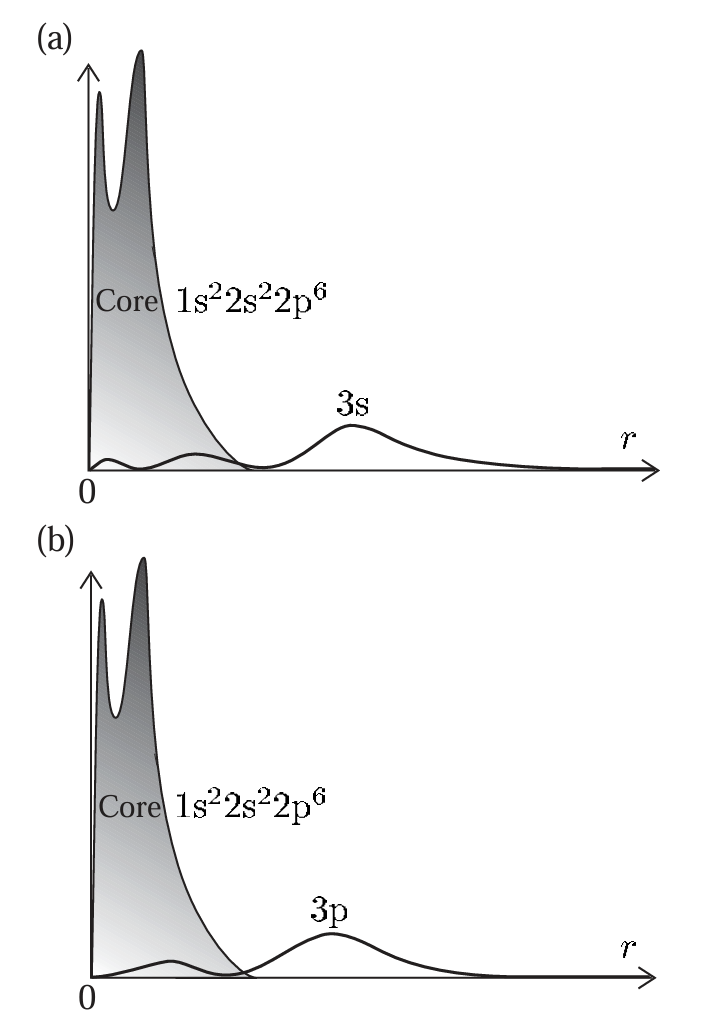
\includegraphics[width=0.3\linewidth]{figs/appB-3.png}
	\caption{不同角量子数 $l$的屏蔽效果}
	\label{fig:appA-2}
\end{figure}

因此，与主量子数相同的氢原子能级相比，碱金属原子的能级更低，这便是\textbf{量子数亏损理论}的核心结论。

对于常见的碱金属原子，它们的主项能量通常位于光学频段，量级大约为 $1\ \mathrm{eV}$。比如 $^{87}\mathrm{Rb}$ 的 $5S_{1/2}\rightarrow5P_{3/2}$ 跃迁的波长大约是 $780\ \mathrm{nm}$。

引入自旋—轨道耦合项 $\hat{H}_\text{SOC}$ 后，能级的简并性会部分解除，形成精细结构分裂。此时，轨道角动量 $\boldsymbol{L}$ 和自旋角动量 $\boldsymbol{S}$ 耦合成总角动量 $\boldsymbol{J}=\boldsymbol{L}+\boldsymbol{S}$，$m_l$ 和 $m_s$ 不再是好量子数，新的好量子数是 $n,l,s,j,m_j$，满足：

\[
\hat{J}^2 \ket{n,l,s,j,m_j} = j(j+1)\hbar^2 \ket{n,l,s,j,m_j},
\]

\[
\hat{J}_z \ket{n,l,s,j,m_j} = m_j \hbar \ket{n,l,s,j,m_j}.
\]

精细结构的能量尺度大约是主能级间隔的 $\alpha^2$（$\alpha$ 为精细结构常数）。我们最熟悉的双线结构就是钠的双黄线，其微小的能量分裂通常处于毫电子伏特（meV）量级。

如果再考虑超精细相互作用 $\hat{H}_\text{HFS}$，核自旋自由度会参与能级的决定。电子的总角动量 $\boldsymbol{J}$ 和核自旋 $\boldsymbol{I}$ 耦合成总角动量 $\boldsymbol{F}=\boldsymbol{I}+\boldsymbol{J}$，此时的好量子数是 $n,l,s,j,I,F,m_F$，满足：

\[
\hat{F}^2 \ket{n,l,s,j,I,F,m_F} = F(F+1)\hbar^2 \ket{n,l,s,j,I,F,m_F},
\]

\[
\hat{F}_z \ket{n,l,s,j,I,F,m_F} = m_F \hbar \ket{n,l,s,j,I,F,m_F}.
\]

超精细分裂的能量尺度比精细结构要小，通常在 GHz 到 MHz 的微波和射频频段。更高精度下，我们还可以观察到兰姆位移等微小的修正，但它们的量级更低，实验中通常不需要考虑。

到这里，我们就能完全理解铷-87的能级图。能级是否分裂完全取决于我们考虑的精度，耦合项的引入意味着两个独立的角动量开始耦合。

从角动量的角度看，这个过程展示了角动量逐步耦合的结构。对于两个独立的角动量 $\boldsymbol{J}_1$ 和 $\boldsymbol{J}_2$，如果它们没有耦合，系统的状态就可以用直积基 $\ket{j_1,m_1}\ket{j_2,m_2}$ 描述；而当它们耦合成总角动量 $\boldsymbol{J}$ 时，应该使用耦合基 $\ket{j_1,j_2;J,M}$ 来描述，二者之间通过 Clebsch–Gordan 系数相联系：

\[
\ket{j_1,j_2;J,M} = \sum_{m_1,m_2} \langle j_1,j_2;m_1,m_2 \vert J,M \rangle \ket{j_1,j_2;m_1,m_2}.
\]

需要注意的是，角动量耦合的方式实际上是由不同相互作用的能量尺度决定的。当某个相互作用远小于主导项时，我们可以把它看作微扰项；而当外加的磁场或电场足够强时，能量尺度的排序会发生变化，体系可能进入强场极限（比如 Paschen–Back 区域），此时原有的耦合近似会失效，角动量也会重新解耦。

因此，分析原子能级结构，本质上是一个根据能量层级逐步展开并不断修正对称性结构的过程。

AMO实验中另一张常用的示意图是塞曼分裂图\ref{fig:appA-3}。

\begin{figure}[htbp]
	\centering
	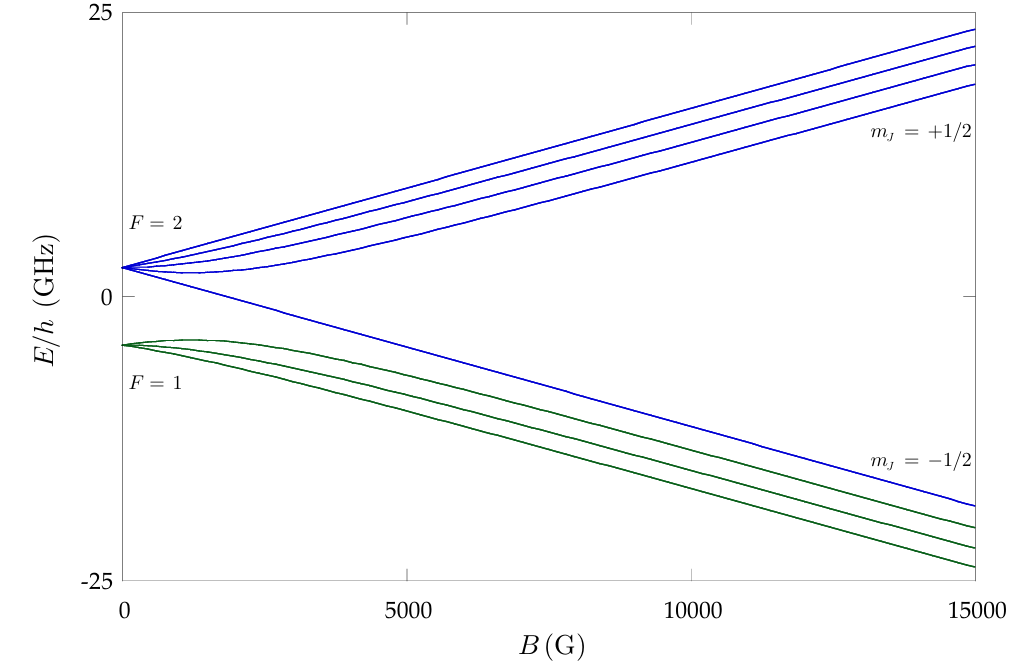
\includegraphics[width=0.6\linewidth]{figs/appB-2.png}
	\caption{铷-87（$^{87}\text{Rb}$）原子的基态塞曼分裂图}
	\label{fig:appA-3}
\end{figure}

在小磁场情况下，$\Delta E_B \ll \Delta E_\text{HFS}$，$\hat{H}_B$ 被当成微扰处理，$I$ 和 $J$ 依然耦合，$m_F$ 仍然是“好”量子数，能级仍然可以用$\ket{n,l,s,j,I,F,m_F}$ 来描述。因此：

\[
\Delta E_B = m_F g_F \mu_B B_z
\]

在弱磁场下，$m_F g_F$ 的符号决定了线性分裂的方向。$m_F = 0$ 的态对磁场不敏感，通常作为\textbf{钟跃迁态}。

在强磁场（Paschen–Back 区域）下，$\Delta E_B \gg \Delta E_\text{HFS}$，$\hat{H}_B$ 不再是微扰，$\hat{H}_\text{HFS}$ 可以被忽略，$I$ 和 $J$ 会解耦，能级用$\ket{n,l,s,j,m_j,I,m_I}$ 来描述，因此，$I$ 和 $J$ 会决定能级分裂的大小和方向。强磁场下，能量分裂的公式为：

\[
\Delta E_B = \dots + \mu_B \bigl( g_J m_J + g_I m_I \bigr) B_z
\]

其中 $g_I \approx -10^{-3}$，而 $g_J \approx 1$。因此，能级分裂的方向主要由 $m_J$ 的符号和大小决定。在强磁场下，$m_J$ 为正的能级会上升，$m_J$ 为负的能级则会下降。

磁光阱和磁阱的理论基础正是基于这个原理，而丰富的内态也为能级操控提供了更多的可能，附录B将介绍辐射场与原子的相互作用。
	%\chapter{辐射场与原子的相互作用}
\section{二能级模型的半经典处理}
\subsection{光学布洛赫方程}
\section{二能级模型的量子处理}
\subsection{J-C模型}
\subsection{缀饰态方法}
\section{跃迁定则}
\section{光对原子的作用力}
	%\chapter{激光稳频}
\section{饱和吸收稳频}
\section{调制转移稳频}
调制转移谱（Modulation Transfer Spectroscopy, MTS）是一种广泛应用于激光稳频的高灵敏光谱技术。其核心思想是通过电光相位调制在激光光场上产生边带，再利用原子的饱和吸收效应将调制信息转移到探测光的幅度上，最终通过解调获得色散型误差信号，实现激光频率对原子跃迁线的锁定。

首先，使用电光调制器（EOM）对频率为 $\omega_0$ 的单频激光进行相位调制。调制后的光场可表示为：
\begin{equation}
	E(t) = E_0 e^{i\left(\omega_0 t + \beta \sin(\Omega_m t)\right)},
\end{equation}
其中 $E_0$ 为光场振幅，$\beta$ 为调制深度，$\Omega_m$ 为调制频率。利用贝塞尔函数恒等式 $e^{i z \sin\theta} = \sum_{n=-\infty}^{\infty} J_n(z) e^{i n \theta}$，可将光场展开为：
\begin{equation}
	E(t) = E_0 \sum_{n=-\infty}^{\infty} J_n(\beta) e^{i\left(\omega_0 + n \Omega_m\right) t},
\end{equation}
其中 $J_n(\beta)$ 为第 $n$ 阶贝塞尔函数。上式表明，相位调制后的激光包含了载波 $\omega_0$ 以及一系列边带 $\omega_0 \pm n \Omega_m$。


将调制后的激光分为两束：**泵浦光**（较强）和**探测光**（较弱），两束光反向传播通过原子/分子样品池。
当激光频率扫描至原子跃迁频率 $\omega_a$ 附近时，强泵浦光会使原子激发态饱和，在多普勒展宽的吸收谱线上“烧”出一个窄孔（饱和吸收效应）。
由于泵浦光带有相位调制边带，其与探测光在原子介质中的非线性相互作用（四波混频过程）会将泵浦光的调制信息转移到探测光的幅度上。此时，探测光不仅经历吸收，其幅度也会携带频率为 $\Omega_m$ 的调制成分。

通过光电探测器探测经过样品池后的探测光，并将信号输入锁相放大器（Lock-in Amplifier），以调制频率 $\Omega_m$ 为参考进行解调。
解调后得到的信号是一个**色散型（Dispersive）误差信号**：
- 当激光频率 $\omega_0 = \omega_a$ 时，误差信号为零；
- 当 $\omega_0 > \omega_a$ 时，误差信号为正；
- 当 $\omega_0 < \omega_a$ 时，误差信号为负。

将此误差信号反馈回激光的频率调谐机构（如压电陶瓷、温度控制器），即可将激光频率稳定在原子跃迁线的中心频率 $\omega_a$ 处。

调制转移谱稳频具有灵敏度高、谱线窄、无多普勒背景等优点，是冷原子物理、量子光学等领域中常用的激光稳频技术。
\section{PDH稳频}
\end{document}